\documentclass{article}

% if you need to pass options to natbib, use, e.g.:
%     \PassOptionsToPackage{numbers, compress}{natbib}
% before loading neurips_2019

% ready for submission
\usepackage{neurips_2019}


% Throughout
\newcommand{\given}{\,|\,}
\newcommand{\compcond}[1]{\big(#1\given-\big)}
\newcommand{\tapprox}{\!\approx\!}
\newcommand{\tequiv}{\!\equiv\!}
\newcommand{\teq}{\!=\!}
\newcommand{\tp}{\!+\!}
\newcommand{\tm}{\!-\!}
\newcommand{\tsim}{\!\sim\!}
\newcommand{\ttimes}{\!\times\!}
\newcommand{\tin}{\!\in\!}

\newcommand{\Eq}[1]{\mathbb{E}_Q\left[#1\right]}
\newcommand{\Vq}[1]{\mathbb{V}_Q\left[#1\right]}
\newcommand{\Gq}[1]{\mathbb{G}_Q\left[#1\right]}
\newcommand{\E}[1]{\mathbb{E}\left[#1\right]}
\newcommand{\V}[1]{\mathbb{V}\left[#1\right]}
\newcommand{\G}[1]{\mathbb{G}\left[#1\right]}
\newcommand{\Gqnot}[2]{\mathbb{G}_{Q_{\backslash #1}}\left[#2\right]}
\newcommand{\Eqnot}[2]{\mathbb{E}_{Q_{\backslash #1}}\left[#2\right]}

% Commands for sampling
\newcommand{\Pois}[1]{\textrm{Pois}\left( #1 \right)}
\newcommand{\Bess}[1]{\textrm{Bessel}\left( #1 \right)}
\newcommand{\Binom}[1]{\textrm{Binom}\left( #1 \right)}
\newcommand{\Gam}[1]{\textrm{Gam}\left( #1 \right)}
\newcommand{\Multi}[1]{\textrm{Multinom}\left( #1 \right)}
\newcommand{\Dirac}[1]{\mathbb{1}\left[ #1 \right]}

% APF
\newcommand{\Yten}{\boldsymbol{Y}}
\newcommand{\osub}{\textrm{i}}
\newcommand{\osubs}{\textbf{\osub}}
\newcommand{\lsubs}{\boldsymbol{\kappa}}
\newcommand{\wsu}[2]{#1_{\subs #2}}
\newcommand{\wsup}[2]{#1_{\subs}^{(#2)}}


\newcommand{\yd}{y_{\osubs}}
\newcommand{\ydk}{y_{\osubs \lsubs}}
\newcommand{\mud}{\mu_{\osubs}}
\newcommand{\mudk}{\mu_{\osubs \lsubs}}
\newcommand{\kappas}{\boldsymbol{\kappa} \in \mathcal{K}}
\newcommand{\sumkappa}{\sum_{\kappas}}


\newcommand{\mask}{b}
\newcommand{\maskten}{\boldsymbol{B}}
\newcommand{\maskd}{\mask_{\osubs}}

\newcommand{\ija}{i {\xrightarrow{a}} j}
\newcommand{\yija}{y_{\ija}}
\newcommand{\maskija}{\mask_{\ija}}

% FROM PrGDS
\newcommand{\ydt}{y^{\mathsmaller{(t)}}_{\osubs}}
\newcommand{\rhot}{\rho^{\mathsmaller{(t)}}}
\newcommand{\thetakt}{\theta_{k}^{\mathsmaller{(t)}}}
\newcommand{\thetakttm}{\theta_{k_2}^{\mathsmaller{(t\!-\!1)}}}
\newcommand{\phikv}{\phi_{kv}}
\newcommand{\epstheta}{\epsilon_0^{\mathsmaller{(\theta)}}}
\newcommand{\epslambda}{\epsilon_0^{\mathsmaller{(\lambda)}}}


\newcommand{\mkt}{m^{\mathsmaller{(t)}}_{k}}
\newcommand{\ykt}{y^{\mathsmaller{(t)}}_{k}}
\newcommand{\yvt}{y^{\mathsmaller{(t)}}_{v}}
\newcommand{\yvtk}{y^{\mathsmaller{(t)}}_{vk}}
\newcommand{\yitk}{y^{\mathsmaller{(t)}}_{\mathbf{v}k}}
\newcommand{\yit}{y^{\mathsmaller{(t)}}_{\mathbf{v}}}
\newcommand{\muitk}{\mu^{\mathsmaller{(t)}}_{\mathbf{v}k}}
\newcommand{\pitk}{p^{\mathsmaller{(t)}}_{\mathbf{v}k}}
\newcommand{\textr}{\textrm{r}}
\newcommand{\thetalam}{\sum_{k_2=1}^K \lambda_{kk_2} \theta_{k_2}^{(t{-}1)}}
\newcommand{\thetapi}{\sum_{k_2=1}^K \pi_{kk_2} \theta_{k_2}^{(t{-}1)}}

\newcommand{\omegakt}{\omega_{k}^{\mathsmaller{(t)}}}
\newcommand{\zetakt}{\zeta_{k}^{\mathsmaller{(t)}}}
\newcommand{\zetaktp}{\zeta_{k}^{(t \tp 1)}}
\newcommand{\deltat}{\delta^{\mathsmaller{(t)}}}
\newcommand{\alphakt}{\alpha_{k}^{\mathsmaller{(t)}}}
\newcommand{\betakt}{\beta_{k}^{\mathsmaller{(t)}}}
\newcommand{\thetaktm}{\theta_{k}^{\mathsmaller{(t\!-\!1)}}}
\newcommand{\thetaktp}{\theta_{k}^{\mathsmaller{(t\!+\!1)}}}
\newcommand{\hkt}{h_k^{\mathsmaller{(t)}}}
\newcommand{\hdkt}{h_{\cdot k}^{\mathsmaller{(t)}}}
\newcommand{\hkdt}{h_{k \cdot}^{\mathsmaller{(t)}}}
\newcommand{\hktm}{h_{k}^{\mathsmaller{(t\!-\!1)}}}
\newcommand{\hktp}{h_{k}^{\mathsmaller{(t\!+\!1)}}}
\newcommand{\hdktp}{h_{\cdot k}^{\mathsmaller{(t\!+\!1)}}}
\newcommand{\hkdtp}{h_{k \cdot}^{\mathsmaller{(t\!+\!1)}}}
\newcommand{\hkkt}{h_{kk_2}^{\mathsmaller{(t)}}}
\newcommand{\phimki}{\phi_{ki_m}^{(m)}}
\newcommand{\alphamki}{\alpha_{ki_m}^{(m)}}
\newcommand{\betamki}{\beta_{ki_m}^{(m)}}
\newcommand{\tildethetakt}{\tilde{\boldsymbol{\theta}}_{k}^{\mathsmaller{(t)}}}
\newcommand{\tildethetaktm}{\tilde{\boldsymbol{\theta}}_{k}^{(t\tm1)}}
\newcommand{\cm}{c^{(m)}}
\newcommand{\ez}{\epsilon_0}
\newcommand{\lkt}{l_k^{\mathsmaller{(t)}}}
\newcommand{\hypconf}[1]{{}_1\textrm{F}_1\left( #1 \right)}


% \newcommand{\prodbeta}{\big(\hspace{-0.25em}\prod_{j \in \mathcal{R}_d}\hspace{-0.25em}\beta_{kj}\big)}
% \newcommand{\prodbetanj}{\big(\hspace{-0.25em}\prod_{j' \in \mathcal{R}_d}\hspace{-0.25em}\beta_{kj'}\big)}
% \newcommand{\lnphi}{\ln(1+\phi_{kv}\,\xi^{-1})}
% \newcommand{\omegarate}{\omega^{(\tau_d)}_{s_d \xrightarrow{k} \mathcal{R}_d}}

% to compile a preprint version, e.g., for submission to arXiv, add add the
% [preprint] option:
    % \usepackage[preprint]{neurips_2019}

% to compile a camera-ready version, add the [final] option, e.g.:
     % \usepackage[final]{neurips_2019}

% to avoid loading the natbib package, add option nonatbib:
%     \usepackage[nonatbib]{neurips_2019}

\PassOptionsToPackage{numbers, compress}{natbib}
\usepackage[utf8]{inputenc} % allow utf-8 input
\usepackage[T1]{fontenc}    % use 8-bit T1 fonts
\usepackage{hyperref}       % hyperlinks
\usepackage{url}            % simple URL typesetting
\usepackage{booktabs}       % professional-quality tables
\usepackage{amsfonts}       % blackboard math symbols
\usepackage{nicefrac}       % compact symbols for 1/2, etc.
\usepackage{microtype}      % microtypography
\usepackage{amsmath}
\usepackage{amssymb} 
\usepackage[capitalise]{cleveref}
% \creflabelformat{equation}{#1#2#3}
% \crefname{equation}{eq.}{eqs.}
% \Crefname{equation}{Eq.}{Eqs.}
\Crefname{section}{\S}{\S}

\usepackage{graphicx,subfigure}
\usepackage{relsize}
\hypersetup{colorlinks,breaklinks,
            allcolors=[rgb]{0.25,0.5,1}}


\title{Poisson-Randomized Gamma Dynamical Systems}

% The \author macro works with any number of authors. There are two commands
% used to separate the names and addresses of multiple authors: \And and \AND.
%
% Using \And between authors leaves it to LaTeX to determine where to break the
% lines. Using \AND forces a line break at that point. So, if LaTeX puts 3 of 4
% authors names on the first line, and the last on the second line, try using
% \AND instead of \And before the third author name.

\author{%
  Aaron Schein \\
  Data Science Institute\\
  Columbia University\\
  % \texttt{hippo@cs.cranberry-lemon.edu} \\
  % examples of more authors
  \And
  Scott Linderman \\
  Data Science Institute\\
  Columbia University\\
  % \texttt{email} \\
  \AND
  Mingyuan Zhou \\
  McCombs School of Business\\
  University of Texas at Austin\\
  % \texttt{email} \\
  \And
  David Blei \\
  Computer Science Department\\
  Columbia University\\
  % \texttt{email} \\
  \And
  Hanna Wallach \\
  Microsoft Research\\
  New York, NY\\
  % \texttt{email} \\
}

\begin{document}

\maketitle

\begin{abstract}
This paper presents the Poisson-randomized gamma dynamical system (PrGDS), a model for sequentially-observed count tensors that encodes a strong inductive bias towards sparsity and burstiness. The PrGDS is based on a new motif in Bayesian latent variable modeling---an alternating chain of discrete Poisson and continuous gamma latent states---that is analytically convenient and computationally tractable, yielding closed-form complete conditionals for all variables by way of the Bessel distribution and a novel discrete distribution that we call the shifted confluent hypergeometric distribution. We draw connections to closely-related models and compare the PrGDS to them in studies of real-world count data of text, international events, and neural spike trains. We find that a sparse variant of the PrGDS---which allows continuous latent states to take values of exactly zero---often obtains the lowest smoothing and forecasting perplexity of all models and is uniquely capable of inferring latent structure that is highly localized in time.~\looseness=-1
\end{abstract}

\section{Introduction}

Political scientists regularly analyze event counts of the number of times country $i$ took action $a$ towards country $j$ during time step $t$ \cite{schrodt1995event}. Such data exhibits ``complex dependence structures'' \cite{king2001proper} like coalitions of countries and bursty temporal dynamics. These dependence structures violate the independence assumptions of traditional regression methods that political scientists have traditionally used to test theories of international relations \cite{green2001dirty,poast2010mis,erikson2014dyadic}. Political scientists have thus advocated for using latent variable models to infer unobserved structure as a way of controlling for it \cite{stewart2014latent}. The latter approach motivates interpretable yet expressive models, capable of capturing a variety of complex latent structures. Event data sets can be represented as a sequence of count tensors $\Yten^{\mathsmaller{(1)}},\dots,\Yten^{\mathsmaller{(T)}}$ each of which contains the $V \ttimes V \ttimes A$ event counts for that time step for every combination of $V$ sender countries, $V$ receivers, and $A$ action types. Recent work applies tensor decomposition methods to event data sets \cite{hoff2004modeling,hoff2015multilinear,schein2015bayesian,hoff2016equivariant,schein2016bayesian}, which infers interpretable coalition structure among countries and topic structure among actions. Like most tensor decomposition methods though, these methods assume that the sequence of tensors is exchangeable and cannot capture the temporal structure in the data.~\looseness=-1  

% In parallel, work on applying deep recurrent neural networks to event data suggests such methods may be effective at forecasting \cite{trivedi2017know}. There is generally a gap in the literature between flexible models useful for prediction and parsimonious models useful for a range of exploratory and explanatory tasks that arise in scientific practice.
% 
Sequentially observed count tensors present unique statistical challenges because they tend to be \emph{bursty} \cite{kleinberg2003bursty}, \emph{high-dimensional}, and \emph{sparse} \cite{chi2012tensors,kunihama2013bayesian}. There are few models that are tailored to both the challenging properties count time-series and count tensors.~\looseness=-1
% Many core tasks within machine learning research begin with count-valued time series, like community detection in dynamic networks, topic modeling in document streams, and time-sensitive recommendation. Count-valued time series frequently exhibit patterns like asymmetry (i.e., they cannot dip below zero) and ``burstiness'' (i.e., sudden and extreme occurrence) that violate the assumptions of traditional time-series models. 
In recent years, Poisson factorization has emerged as a framework for modeling sparse count matrices~\cite{canny2004gap,Dunson2005bayesianlatent,titsias2008infinite,cemgil2009bayesian,zhou2011beta,gopalan2013efficient} and tensors \cite{chi2012tensors,ermis2014bayesian,schein2015bayesian}. While tensor decomposition methods generally scale with the size the tensor, many Poisson factorization models yield inference algorithms that scale linearly with only the non-zeros. This property allows researchers to efficiently explore latent structure in massive tensors, provided they are sparse. However, this property is unique to a subset of Poisson factorization models that only use non-negative prior distributions, which are difficult to chain in state-space models for time series. Hierarchical compositions of non-negative priors---notably, the gamma and Dirichlet---typically introduce non-conjugate dependencies that require innovative posterior schemes.\looseness=-1

% to build such models for complex dependence structures like time series, researchers must therefore construct structured priors without relying on the convenience and analytic tractability of the Gaussian distribution.

\begin{figure*}[t]
\centering
\subfigure[Poisson--gamma dynamical systems~\cite{schein2016poisson}]
{\label{fig:pgds}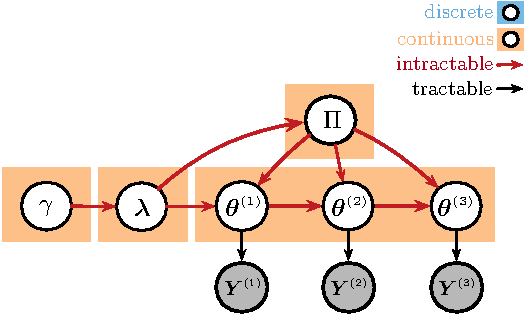
\includegraphics[width=0.49\linewidth]{../../fig/graphical_models/pgds.pdf}}\hfill
% 
\subfigure[Poisson-randomized gamma dynamical systems]
{\label{fig:prgds}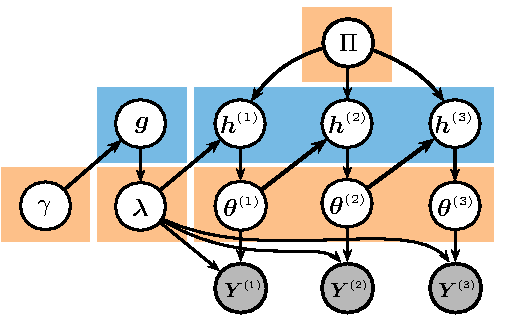
\includegraphics[width=0.49\linewidth]{../../fig/graphical_models/prgds.pdf}}
\caption{\label{fig:comparison} \footnotesize \emph{Left}: The PGDS imposes dependencies directly between the continuous variables that do not yield closed-form conditional distributions. \emph{Right}: The PrGDS (this paper) breaks the intractable dependencies with discrete Poisson variables---doing so yields closed-form conditionals for all variables without any data augmentation.~\looseness=-1}\vspace{-1.5em}
\end{figure*}

This paper seeks to fill a gap in the literature between Poisson factorization models that are \emph{tractable}---i.e., yielding closed-form complete conditionals that make approximate inference easy to derive---and those that are \emph{expressive}---i.e., capable of capturing a variety of complex dependence structures. To do so, we introduce alternating chains of discrete Poisson and continuous gamma latent states, a new modeling motif that is analytically convenient and computationally tractable. We rely on this motif to construct the Poisson-randomized gamma dynamical system (PrGDS), a model for sequentially observed count tensors that is tractable, expressive, and efficient. The PrGDS is closely related to the Poisson--gamma dynamical system (PGDS) \cite{schein2016poisson}, a recently introduced model for dynamic count matrices, that is based on non-conjugate chains of gamma-distributed states. These chains are intractable---thus, posterior inference in the PGDS relies on sophisticated data augmentation schemes that are cumbersome to derive and impose unnatural restrictions on the priors over other variables. The PrGDS instead introduces intermediate Poisson states that break the intractable dependency between the gamma states (see \cref{fig:comparison}). While this construction is only \emph{semi}-conjugate, it is tractable, yielding closed-form complete conditionals for the Poisson states by way of the little-known Bessel distribution~\cite{yuan2000bessel} and a novel discrete distribution that we derive and call the \emph{shifted confluent hypergeometric (SCH) distribution}.~\looseness=-1

We study the inductive bias of the PrGDS by comparing its smoothing and forecasting ability to the PGDS and two other baselines on a range of real-world count matrices and tensors of text, international events, and neural spike data. We find that the PrGDS often obtains lower smoothing and forecasting perplexity than the PrGDS and related baselines. The PrGDS under a specific hyperparameter setting permits the continuous states to take values of \emph{exactly} zero thus encoding a unique inductive bias tailored to sparsity and burstiness. We find that this variant, in particular, often obtains the lowest perplexity of all models. We also find that the sparse PrGDS infers a qualitatively broader range of latent structure---specifically, bursty latent structure that is highly localized in time.~\looseness=-1

% We present the PrGDS in \cref{sec:prgds} and detail its connections to prior work in \cref{sec:bg}. In \cref{sec:mcmc}, we show that PrGDS admits closed-form complete conditionals for all variables without any data augmentation. To do so, in \cref{sec:recursion}, we discuss and derive identities about the general motif on which PrGDS is based. In \cref{sec:empirical}, we study the inductive bias of the PrGDS by comparing its smoothing and forecasting ability to the PGDS and two other baselines on a range of real-world count matrices and tensors of text, international events, and neural spike data. We find that the PrGDS often obtains lower smoothing and forecasting perplexity than the PrGDS and related baselines. The PrGDS under a specific hyperparameter settings permits the continuous states to take values of \emph{exactly} zero thus encoding a unique inductive bias tailored to sparsity and burstiness. We find that this variant, in particular, often obtains the lowest perplexity of all models and additionally infers qualitatively different latent structure that is highly localized in time.~\looseness=-1

% Beyond political science, sequentially observed count tensors are the object of analysis in many scientific disciplines. Neuroscientists, for instance, apply tensor decomposition methods to tensors of neuron spike counts to infer interpretable structure that can be explored to suggest new scientific theories about animal behavior and cognition \cite{williams2018unsupervised}. 

% In addition to being uniquely capable of inferring highly localized latent structure, 
% \pagebreak
\section{Poisson-randomized gamma dynamical systems (PrGDS)}
\label{sec:prgds}

\textbf{Notation.} Consider a data set of of sequentially observed tensors $\boldsymbol{Y}^{\mathsmaller{(1)}},\dots,\boldsymbol{Y}^{\mathsmaller{(T)}}$. An entry $\ydt \!\in\! \{0,1,2,\dots\}$ in the $t^{\textrm{th}}$ tensor is subscripted by a multi-index $\osubs \equiv (\osub_1,\dots,\osub_M)$ which indexes into the $M$ modes of the tensor. As an example, international event counts $y^{\mathsmaller{(t)}}_{\mathsmaller{i \xrightarrow{a} j}}$ of the number of times country $i$ took action $a$ to country $j$ during time step $t$, can be rewritten as $\ydt$  where the multi-index corresponds to a unique combination of sender, receiver, and action type---i.e., $\osubs = (i, j, a)$.~\looseness=-1

\textbf{Generative process.} The PrGDS is a form of canonical polyadic decomposition \cite{harshman1970foundations} that models $\yd$ as~\looseness=-1
\begin{align}
\label{eq:tensor_likelihood}
\ydt &\sim \textrm{Pois}\Big(\rhot \sum_{k = 1}^K \lambda_k \, \thetakt \prod_{m=1}^M \phi^{\mathsmaller{(m)}}_{k \osub_m}\Big).
\end{align}
Here $\thetakt$ represents the activation of the $k^{\textrm{th}}$ \emph{component} at time step $t$. Each component describes a dependence structure in the data by way of a factor vector $\boldsymbol{\phi}^{\mathsmaller{(m)}}_{k}$ for each mode $m$. For international events data, the first factor vector $\boldsymbol{\phi}^{\mathsmaller{(1)}}_{k} \teq (\phi^{\mathsmaller{(1)}}_{k1},\dots,\phi^{\mathsmaller{(1)}}_{kV})$ describes the rate at which each of the $V$ countries acts as a sender in the $k^{\textrm{th}}$ component while the second $\boldsymbol{\phi}^{\mathsmaller{(2)}}_{k}$ describes the rate at which each acts as a receiver. The weights $\lambda_k$ and $\rho^{\mathsmaller{(t)}}$ represent the overall scale of component $k$ and time step $t$. The PrGDS is called \emph{stationary} if $\rhot \teq \rho$. We posit the following conjugate priors,~\looseness=-1
% there is a set of factors $\phi^{\mathsmaller{(m)}}_{k \osub_m}$ for each mode $m$ that represents the strength of feature $i_{m}$ in component $k$. An analogous generalization can be made of the PGDS. However, as before, the ``augment-and-conquer'' inference is only available if $\lambda_k=\lambda$ and $\sum_{i_m=1}^{L_m} \phi^{\mathsmaller{(m)}}_{k \osub_m} \teq 1$ for all $m$. A secondary contribution of this paper is the generalization of the PGDS to tensor-valued time series which we use in \cref{sec:empirical} as a baseline. We provide the relevant inference equations in the Appendix and will open source our Cython implementation.
\begin{equation}
\rhot \sim \Gam{a_0, b_0} \,\,\,\textrm{ and }\,\,\, \boldsymbol{\phi}^{\mathsmaller{(m)}}_k \sim \textrm{Dir}(a_0,\dots,a_0).
\end{equation}
The PrGDS is characterized by an alternating series of discrete and continuous latent states. The \emph{continuous latent states} $\thetakt$ evolve via intermediate discrete states $\hkt$ from $t=1,\dots,T$ as~\looseness=-1
\begin{equation}
\label{eq:thetaktandhkt}
\thetakt \sim \Gam{\epstheta \tp \hkt,\, \tau} \,\,\textrm{ and }\,\, \hkt \sim \textrm{Pois}\Big(\tau \sum_{k_2 = 1}^K \pi_{kk_2} \,\thetakttm\Big),
\end{equation}
where for $t\teq 0$ we define $\theta^{\mathsmaller{(0)}}_k \teq \lambda_k$ to be the per-component weight that also appears in \cref{eq:tensor_likelihood}. The PrGDS assumes $\thetakt$ is conditionally gamma distributed with \emph{rate} $\tau$ and shape equal to a latent count $\hkt$ plus hyperparameter $\epstheta \geq 0$. We adopt the convention that a gamma random variable is zero, almost surely, if its shape parameter is zero---thus, setting $\epstheta \teq 0$ defines the \emph{sparse PrGDS} wherein the continuous states are exactly zero $\thetakt \stackrel{\textrm{a.s.}}{=} 0$ if $\hkt \teq 0$.

The \emph{transition weights} $\pi_{kk_2}$ in the Poisson rate of $\hkt$ represent how strongly each component $k_2$ excites component $k$ at the subsequent time step. We view these weights collectively as a $K \!\times\! K$ transition matrix $\Pi$ and impose Dirichlet priors over its columns. We also place a gamma prior over the \emph{concentration parameter} $\tau$ which is conjugate to both the gamma and Poisson distributions it appears in:~\looseness=-1
\begin{equation}
\tau \sim \Gam{\alpha_0, \alpha_0} \,\,\textrm{ and }\,\,
\boldsymbol{\pi}_k \sim \textrm{Dir}\left(a_0,\dots,a_0\right) \textrm{ such that }\mathsmaller{\sum_{k_1}}^K \pi_{k_1k}=1.
\end{equation}
% \begin{align}
% \mathbb{E}\left[\boldsymbol{\theta}^{\mathsmaller{(t)}} \given \boldsymbol{\theta}^{\mathsmaller{(t \tm 1)}}\right] = \mathbb{E}\left[\mathbb{E}\left[\boldsymbol{\theta}^{\mathsmaller{(t)}} \given \boldsymbol{h}^{\mathsmaller{(t \tm 1)}}\right]\right] = \Pi \, (\boldsymbol{\theta}^{\mathsmaller{(t \tm 1)}} \odot \boldsymbol{\eta}) 
% \end{align}
% When $\epstheta > 0$, this construction corresponds to the \emph{randomized gamma of the first type}~\citep{yuan2000bessel,makarov2010exact} while when $\epstheta=0$ this construction corresponds to the Poisson-randomized gamma distribution~\citep{zhou2016augmentable}.
% Thus, $\tau$ mainly controls the variance of the latent dynamics while only affecting the expectation by a factor of $\epstheta$ (and not at all when $\epstheta \teq 0$). We impose the  prior $\tau \sim \Gam{\alpha_0, \alpha_0}$ which is conjugate to both the Poisson and gamma distributions in which $\tau$ appears.
For the per-component weights $\lambda_k$, we place a hierarchical prior with a similar flavor to \cref{eq:thetaktandhkt}:~\looseness=-1 
\begin{equation}
\label{eq:lambdakandgk}
\lambda_k \sim \textrm{Gam}\Big(\tfrac{\epslambda}{K} + g_k,\, \beta\Big) \,\,\textrm{ and }\,\,g_k \sim \Pois{\tfrac{\gamma}{K}},
% 
\end{equation}
where $\epslambda$ is a hyperparameter analogous to $\epstheta$. The following gamma priors are then both conjugate:~\looseness=-1
\begin{equation}
\gamma \sim \Gam{a_0,b_0} \,\,\,\textrm{ and }\,\,\, \beta \sim \Gam{\alpha_0, \alpha_0}.
\end{equation}
The PRGDS has five fixed hyperparameters $\epstheta,\epslambda,\alpha_0,a_0,$ and $b_0$. For the empirical studies in \cref{sec:empirical}, we set $a_0\teq b_0 \teq 0.01$ to define weakly informative gamma and Dirichlet priors and $\alpha_0 \teq 10$ to define a gamma prior that promotes values close to 1. We consider two variants for $\epstheta \in \{0,1\}$ with $\epslambda \teq 1$.~\looseness=-1

\textbf{Properties.}
Both $\epslambda$ and $\gamma$ are divided by the number of components $K$ in \cref{eq:lambdakandgk}---as the number of components grows $K \!\rightarrow\! \infty$, the expected sum of the weights thus remains finite and fixed:~\looseness=-1
\begin{equation}
\sum_{k=1}^\infty \E{\lambda_k} = \sum_{k=1}^\infty \big(\tfrac{\epslambda}{K} + \E{g_k}\big) \beta^{-1} = \sum_{k=1}^\infty \big(\tfrac{\epslambda}{K} + \tfrac{\gamma}{K} \big)\beta^{-1} = \big(\epslambda + \gamma \big)\beta^{-1}.
\end{equation}
Thus, this prior encodes an inductive bias towards small values of $\lambda_k$ and may be interpreted as the finite truncation of a novel Bayesian nonparametric process. A small value of $\lambda_k$ shrinks the Poisson rates of both the data $\ydt$ and the first discrete latent state $h^{\mathsmaller{(0)}}_k$---this prior encourages the model to only infer components that are both predictive of the data and useful for fitting the latent dynamics.~\looseness=-1

The marginal expectation of the state vector $\boldsymbol{\theta}^{\mathsmaller{(t)}}$ takes the canonical form of linear dynamical systems,~\looseness=-1
\begin{align}
\label{eq:expectation}
\mathbb{E}\left[\boldsymbol{\theta}^{\mathsmaller{(t)}} \given \boldsymbol{\theta}^{\mathsmaller{(t \tm 1)}}\right] = \mathbb{E}\left[\mathbb{E}\left[\boldsymbol{\theta}^{\mathsmaller{(t)}} \given \boldsymbol{h}^{\mathsmaller{(t \tm 1)}}\right]\right] = \epstheta \tau^{-1} + \Pi \, \boldsymbol{\theta}^{\mathsmaller{(t \tm 1)}},
\end{align}
since by iterated expectation $\E{\thetakt} \teq \big(\epstheta \tp \E{\hkt}\big)\tau^{-1} \teq \big(\epstheta \tp \tau \sum_{k_2 = 1}^K \pi_{kk_2} \,\thetakttm \big) \tau^{-1}$. The \emph{concentration parameter} $\tau$ appears in both the Poisson and gamma distributions in \cref{eq:thetaktandhkt}. It contributes to the variance of the process while canceling out of the expectation, except for the additive term $\epstheta \tau^{-1}$ which vanishes when $\epstheta \teq 0$.

We can analytically marginalize out all of the discrete latent states $\hkt$ to obtain a purely continuous dynamical system. When $\epstheta > 0$, this system can be written in terms of the \emph{randomized gamma distribution of the first type} (RG1) \cite{yuan2000bessel,makarov2010exact},~\looseness=-1
\begin{equation}
\label{eq:rg1}
\
\thetakt \sim \textrm{RG1}\Big(\epstheta,\,\tau\sum_{k_2=1}^K \pi_{kk_2} \thetakttm,\, \tau\Big),
% 
% \,\,\textrm{ such that }\,\, \mathbb{E}\left[\boldsymbol{\theta}^{\mathsmaller{(t)}} \given \boldsymbol{\theta}^{\mathsmaller{(t \tm 1)}}\right] = \tfrac{\epstheta}{\tau} + \Pi \, \boldsymbol{\theta}^{\mathsmaller{(t \tm 1)}}.
\end{equation}
and in terms of a limiting form of the RG1 when $\epstheta \teq 0$. We describe the RG1 distribution in \cref{fig:rg1}.~\looseness=-1

% \pagebreak
\section{Related work}
\label{sec:bg}
\begin{figure}[t]
\centering
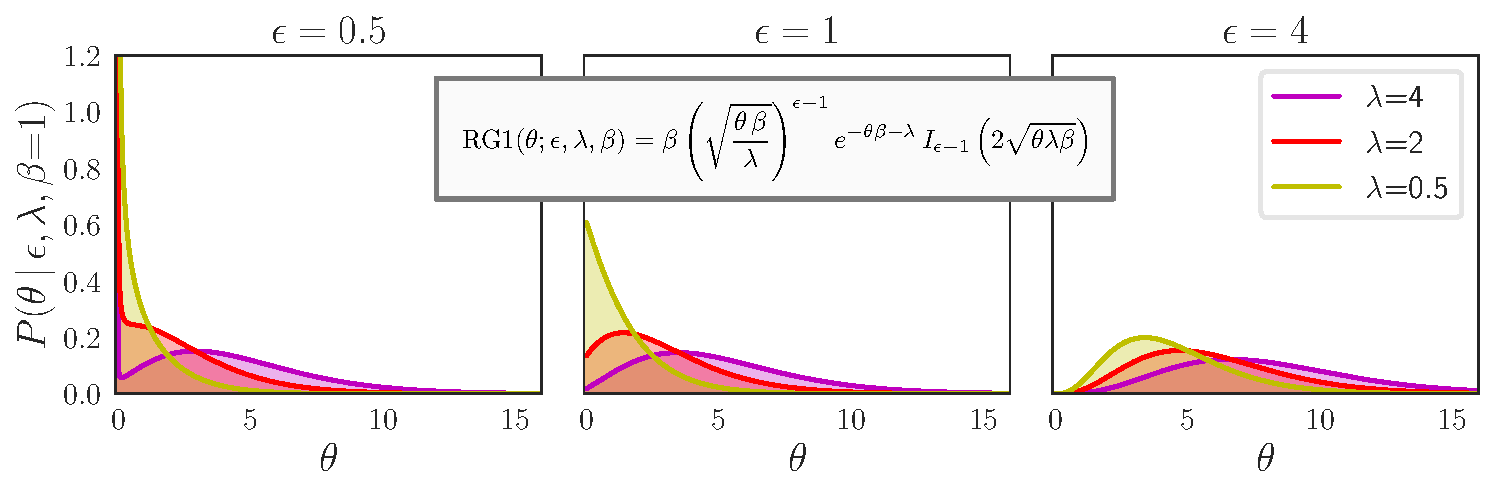
\includegraphics[width=\linewidth]{../../fig/distributions/annotated_rg1.pdf}
\caption{\footnotesize \label{fig:rg1} The randomized gamma distribution of the first type (RG1) \cite{yuan2000bessel,makarov2010exact} has support $\theta \!>\!  0$ and is defined by three parameters $\epsilon,\lambda,\beta \!>\! 0$. Its PDF is given in the plot where $I_{\nu}(a)$ is the modified Bessel function of the first kind \cite{abramowitz1965handbook}. When $\epsilon < 1$ (\emph{left}) the RG1 resembles a soft ``spike-and-slab'' while when $\epsilon \geq 1$ (\emph{middle and right}) it resembles a more-dispersed form of the gamma distribution. A limiting case of the RG1 when $\epsilon \!\rightarrow\! 0$ is the Poisson-randomized gamma distribution \cite{zhou2016augmentable} which includes zeros in its support $\theta \geq 0$.~\looseness=-1}\vspace{-0.5em}
\end{figure}
The PrGDS closely relates to the Poisson--gamma dynamical system (PGDS)~\citep{schein2016poisson} wherein~\looseness=-1\vspace{-0.2em}
\begin{equation}
\label{eq:pgds}
\thetakt \sim \textrm{Gam}\Big(\tau\,\sum_{k_2=1}^K \pi_{kk_2} \thetakttm,\, \tau\Big)\,\,\textrm{ such that }\,\,
% 
\mathbb{E}\left[\boldsymbol{\theta}^{\mathsmaller{(t)}} \given \boldsymbol{\theta}^{\mathsmaller{(t \tm 1)}}\right]= \Pi \, \boldsymbol{\theta}^{\mathsmaller{(t \tm 1)}}.
\end{equation}
The PGDS posits non-conjugate dependence between gamma-distributed states. The complete conditional $P(\thetakt | -)$ is not available in closed form and posterior inference relies on a sophisticated data augmentation scheme. The PrGDS instead introduces intermediate Poisson states $\hkt$ that break the intractable dependencies between the gamma states---we visualize this in \cref{fig:comparison}. While the Poisson distribution is not a conjugate prior to the gamma rate parameter, this construction is still tractable, yielding a closed-form conditional $P(\hkt | -)$, as we'll show in \cref{sec:mcmc}. The PGDS is limited by the data augmentation scheme it requires for posterior inference---specifically, this augmentation scheme does not allow any per-component weights $\lambda_k$ to appear in the Poisson rate of $\ydt$ in \cref{eq:tensor_likelihood}. To encourage parsimony, the PGDS instead draws weights $\lambda_k \sim \textrm{Gam}(\tfrac{\gamma}{K}, \beta)$ and uses them to shrink the transition matrix $\Pi$. This introduces more intractable dependencies that necessitate a different augmentation scheme for inference. These augmentation schemes additionally impose restrictions that the factors $\boldsymbol{\phi}_k^{\mathsmaller{(m)}}$ and columns $\boldsymbol{\pi}_k$ of the transition matrix are Dirichlet distributed---while we adopt those same assumptions in this paper, the PrGDS is not bound to them.~\looseness=-1

The PGDS and its ``deep'' variants~\cite{gong2017deep,guo2018deep} generalize gamma process dynamic Poisson factor analysis (GP-DPFA)~\citep{acharya2015nonparametric} which assumes a simple random walk $\thetakt \tsim \Gam{\theta^{\mathsmaller{(t \tm 1)}}_k,\, c^{\mathsmaller{(t)}}}$; see also a related model~\cite{yang2018dependent}. These models belong to a line of work exploring the application of the ``augment-and-conquer'' data augmentation scheme~\cite{zhou2012augment-and-conquer} to perform inference in hierarchies of gamma variables chained via their shape and linked to Poisson observations---beyond time-series models, this construction can be used to build belief networks~\cite{zhou2015poisson}. An alternative approach is to chain gamma variables via their rate---e.g., $\theta^{\mathsmaller{(t)}} \sim \Gam{a,\,\theta^{\mathsmaller{(t\tm 1)}}}$. This motif is conjugate and tractable and has been applied to time-series models~\cite{cemgil2007conjugate,fevotte2013non,jerfel2016dynamic} and deep belief networks~\cite{ranganath2015deep}. However, unlike the shape, the rate contributes to the variance of the gamma quadratically; rate chains may thus be highly volatile.~\looseness=-1

More broadly, gamma shape and rate chains are examples of non-negative chains. Such chains are particularly motivated in the context of Poisson factorization, which is particularly efficient when only non-negative prior distributions are used. In general, Poisson factorization assumes that each observed count is drawn $\yd \sim \Pois{\mud}$ with latent rate $\mud$ defined to be some function of model parameters. When the rate is linear---i.e., $\mud \teq \sum_{k}\mu_{\osubs k}$---Poisson factorization yields a \emph{latent source representation}~\cite{Dunson2005bayesianlatent,cemgil2009bayesian} wherein we define $\yd \triangleq \sum_k y_{\osubs k}$ to be the sum of latent sources, each of which is drawn $y_{\osubs k} \sim \Pois{\mu_{\osubs k}}$. Conditioning on the latent sources often induces conditional independences between the latent variables and parameters that facilitates closed-form, efficient, and parallelizable posterior inference---thus, the first step in either MCMC or variational inference is to update the latent sources from their complete conditionals, which is multinomial \cite{steel1953relation}~\looseness=-1,
\begin{equation}
\label{eq:thinning}
\compcond{(y_{\osubs1},\dots,y_{\osubs K})} \sim \Multi{\yd,\, (\mu_{\osubs 1},\dots, \mu_{\osubs K})},
\end{equation}
where we leave implicit the normalization of the non-negative rates $\mu_{\osubs k}$ into a probability vector. When the observed count is zero $\yd \teq 0$, the sources are zero $y_{\osubs k} \stackrel{\textrm{a.s.}}{=}0$ and no computation is required to update them. Thus, any Poisson factorization model that admits a latent source representation scales linearly with only the non-zero counts in the data. This property is indispensable when modeling count tensors which typically contain exponentially more zeros than non-zeros~\cite{bhattacharya2012simplex}. 

Since the latent source representation is only available when the rate $\mud$ is a linear function of parameters and since the rate must be non-negative, by definition of the Poisson distribution, efficient Poisson factorization is only compatible with non-negative priors over parameters. Modeling time series and other complex dependence structures with efficient Poisson factorization often requires developing novel motifs that notably exclude Gaussian priors which researchers have traditionally relied on for their analytic convenience and tractability. The Poisson LDS~\cite{smith2003estimating, paninski2010new, macke2011empirical}, for instance, links the widely-used Gaussian linear dynamical system~\cite{kalman1961new,ghahramani1999learning} to  Poisson observations via an exponential link function $\mud = \exp\left({\sum_k \cdots}\right)$. This is one instance of the generalized linear model (GLM) \cite{nelder1972generalized} approach that relies on a non-linear link function and thus does not yield a latent source representation. Another approach is to use log-normal priors, as in Dynamic Poisson Factorization \cite{charlin2015dynamic}---while this approach satisfies the non-negative constraint, the log-normal is not conjugate to the Poisson and does not yield closed-form conditionals. 

There is also a long tradition of autoregressive models for count time series including VAR models~\cite{brandt2012bayesian} and those based on Hawkes processes \cite{hawkes1971spectra,blundell2012modelling,simma2012modeling,linderman2014discovering}. This approach avoids the challenge of constructing tractable state-space models from non-negative priors by modeling temporal correlation directly between the count observations. However, for high-dimensional data, such as sequentially-observed tensors, an autoregressive approach is often untenable.~\looseness=-1 

% As efficient Poisson factorization is  renewed interest \cite{cemgil2019bayesian}, the 

% The PGDS is thus incompatible with gamma priors over the factors $\phi_{kv}$ which are widely used in practice \cite{cemgil2009bayesian,gopalan2015scalable,schein2015bayesian}. It is also incompatible with per-component weights $\lambda_k$ that are widely used in conjunction with Bayesian nonparametric shrinkage priors for implicit model selection \cite{acharya2015nonparametric,schein2016bayesian}. 

% The concentration parameter $\tau$ in the PGDS is analogous to $\tau$ in the PrGDS in that it affects the variance of the latent dynamics without affecting the expected value. However, unlike in the PrGDS, it is treated as a fixed hyperparameter in the PGDS, since no natural conjugate prior exists when it appears in both the shape and rate of the gamma distribution.



% \section{Background}
% \label{sec:bg}



% The challenge we embrace in this paper is thus to construct expressive and structured priors from only non-negative distributions. A reasonable approach is to use the log-normal as a prior, as in Dynamic Poisson factorization~\cite{charlin2015dynamic}. A more natural approach is to use gamma and Dirichlet priors, which are conjugate to the Poisson distribution and yield analytically closed-form complete conditionals. 

% We take a new approach in this paper. Instead of chaining gamma random variables directly, we introduce alternating chains of conditionally gamma- and Poisson- distributed states. This construction is \emph{semi}-conjugate yet yields closed-form complete conditionals for all states, as we show in \cref{sec:mcmc}.\looseness=-1



% Allocative Poisson matrix factorization \cite{canny2004gap,Dunson2005bayesianlatent,titsias2008infinite,cemgil2009bayesian,zhou2011beta,gopalan2013efficient,paisley2014bayesian}. 

% Non-negative tensor decomposition \citep{cichocki2007non,kolda2009tensor} and probabilistic Poisson tensor decomposition \cite{chi2012tensors}, and Bayesian variants \cite{ermis2014bayesian,schein2015bayesian,schein2016bayesian}.

% See \cite{cemgil2019bayesian} for a review of this area along with connections.

% This family of models is underdeveloped due to the lack of tractable and convenient modeling motifs using only non-negative priors. We introduce a fundamentally novel motif and build a dynamical system with it that uses it to chain together dynamic latent states and uses it to shrink.  


% Models that are not tailored to count data fail to make this distinction and thus tend to waste computation and statistical power on the exponentially-large number of zeros, as if each were as informative as a non-zero observation.


\section{Posterior inference}
\label{sec:mcmc}
The complete conditionals for all latent variables in the PrGDS are immediately available in closed form without any data augmentation. Iteratively re-sampling each variable from its conditional constitutes a Gibbs sampling algorithm. We provide conditionals for the latent variables with non-standard priors here and relegate the rest to the Appendix. The PrGDS is based on a new modeling motif---we first introduce it in its general form, derive its conditionals, and then apply these identities to the PrGDS.~\looseness=-1

\subsection{Poisson--gamma--Poisson recursions}
\label{sec:recursion}
Consider the following model of $m$ involving latent variables $\theta$ and $h$ and fixed $c_1, c_2, c_3, \epstheta >0$:
\begin{equation}
m \sim \Pois{\theta c_3},\,\,
% 
\theta \sim \Gam{\epstheta \tp h, c_2},\,\,
% 
\textrm{and}\,\, h \sim \Pois{c_1}.
\end{equation}
This model is \emph{semi}-conjugate. The gamma prior of $\theta$ is conjugate to the Poisson and its posterior is
%
\begin{align} 
\label{eq:gamma}
\compcond{\theta} &\sim \Gam{\epstheta \tp h + m,\, c_2 + c_3}.
% 
\intertext{The Poisson prior over $h$ is not conjugate to the gamma--- however the conditional posterior of $h$ is still available in closed form by way of the Bessel distribution \cite{yuan2000bessel} which we define in \cref{fig:bessel}:}
%
\label{eq:bessel}
\compcond{h} &\sim \textrm{Bes}\big(\epstheta \tm 1,\, 2\sqrt{\theta \,c_2\, c_1}\big).
\end{align}
The Bessel distribution can be sampled efficiently \cite{devroye2002simulating}; we have provided our Cython implementation. 
Provided that $\epstheta \!>\! 0$, sampling $\theta$ and $h$ iteratively from \cref{eq:gamma,eq:bessel} constitutes a valid Markov chain for posterior inference. When $\epstheta \teq 0$ though, $\theta \stackrel{\textrm{a.s.}}{=} 0$ if $h \teq 0$, and vice versa---thus, this Markov chain has an absorbing condition at $h \teq 0$ and violates detailed balance. In this case, we must therefore sample $h$ with $\theta$ marginalized out---towards that end, we prove Theorem 1.~\looseness=-1

\textbf{Theorem 1:} \textit{The incomplete conditional $P(h\given{\epstheta \teq 0, -\backslash} \theta)\triangleq \int P(h,\theta\given \epstheta \teq 0, -)\,\mathbf{d}\theta$ is}~\looseness=-1
\begin{align}
\label{eq:sch}
\left(h \given {-\backslash} \theta\right) &\sim
\begin{cases}
\textrm{Pois}\big(\frac{c_1\,c_2}{c_3+c_2}\big) &\textrm{if }m=0\\
\textrm{SCH}\big(m,\, \frac{c_1\,c_2}{c_3+c_2}\big)\, &\textrm{otherwise}
\end{cases}
\end{align}
\textit{where SCH is a discrete distribution we call the shifted confluent hypergeometric distribution. We describe the SCH in \cref{fig:sch} and provide further details about it in the Appendix including the derivation of its PMF, PGF, and mode, along with details of how we sample from it and the proof for Theorem 1.}~\looseness=-1

\begin{figure*}[t]
\centering
\subfigure[\footnotesize Bessel distribution.~\cite{yuan2000bessel}]
{\label{fig:bessel}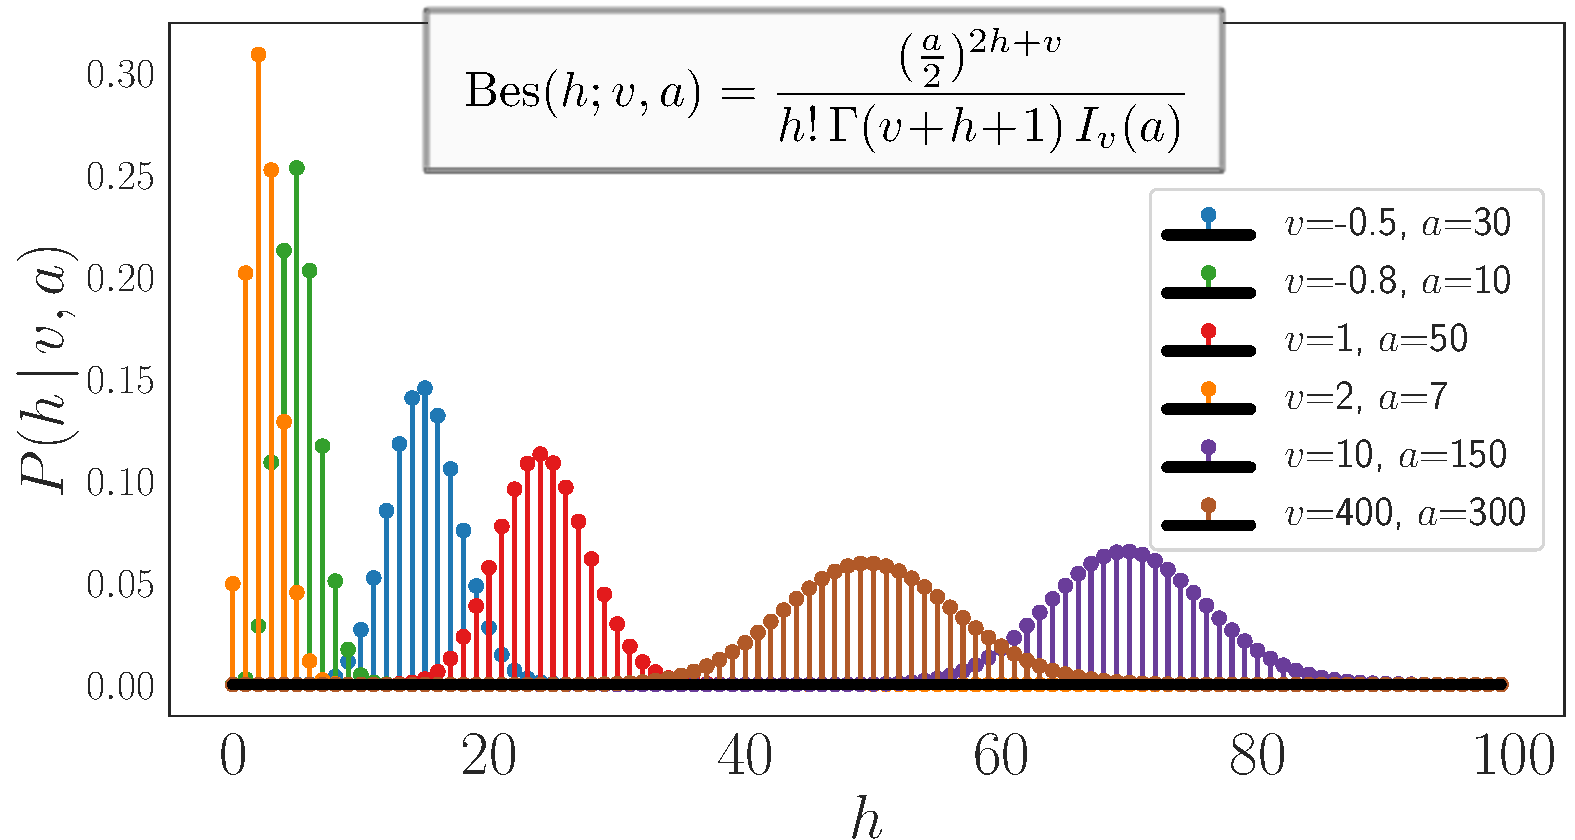
\includegraphics[width=0.5\linewidth]{../../fig/distributions/annotated_bessel.pdf}}\hfill
% 
% \hspace{0.5em}
\subfigure[\footnotesize Shifted confluent hypergeometric (SCH) distribution]
{\label{fig:sch}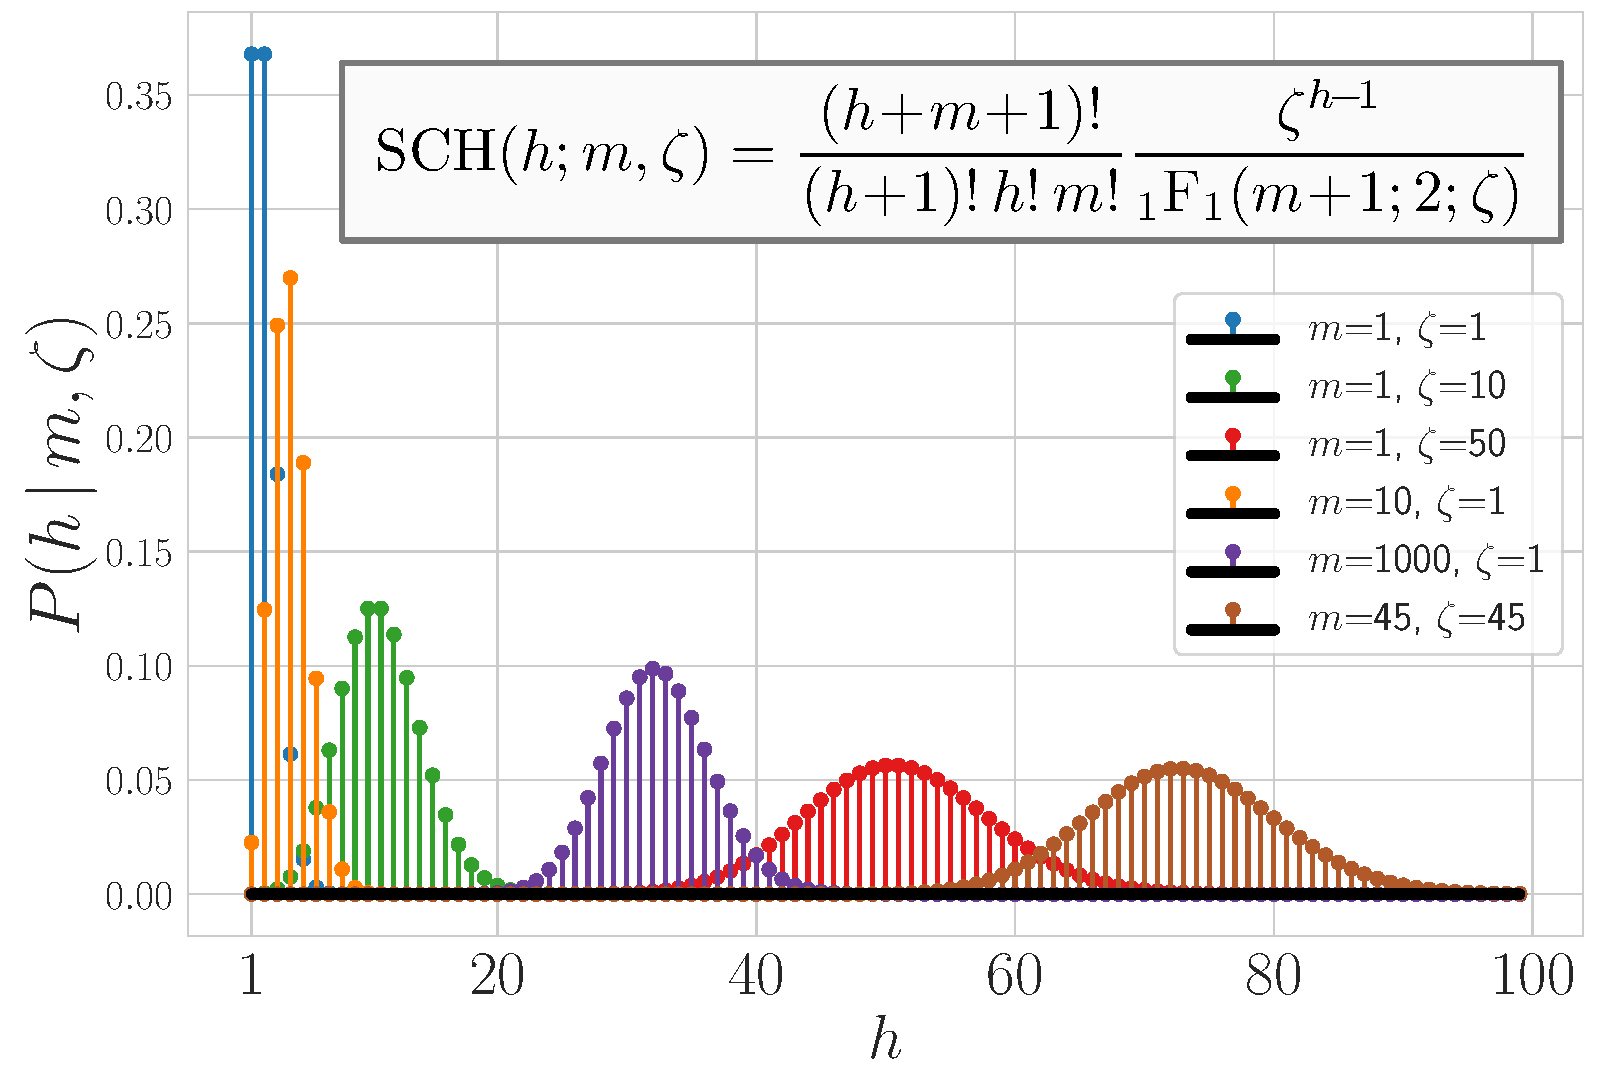
\includegraphics[width=0.5\linewidth]{../../fig/distributions/annotated_sch.pdf}}\vspace{-0.5em}
\caption{\footnotesize \label{fig:distributions} Two discrete distributions that arise as posteriors in Poisson--gamma--Poisson recursions.~\looseness=-1}\vspace{-1em}
\end{figure*}

\subsection{Closed-form complete conditionals for the PrGDS}
The PrGDS yields a latent source representation (see \cref{eq:thinning})---posterior inference begins with
\begin{align}
\compcond{(y^{\mathsmaller{(t)}}_{\osubs k})_{k=1}^K} &\sim \Multi{\ydt,\big(\lambda_k \, \thetakt \mathsmaller{\prod}_{m=1}^M \phimki\big)_{k=1}^K}.
\intertext{We may similarly represent $\hkt$ under its latent source representation as $\hkt \tequiv \hkdt \teq \sum_{k_2=1}^K \hkkt$ where $\hkkt \tsim \Pois{\tau \, \pi_{kk_2} \thetakttm}$. When useful, we use dot-notation (``$\bcdot$'') to denote summing over an axis---in this case $\hkdt$ denotes the sum of the $k^{\textrm{th}}$ row of the $K \ttimes K$ matrix of latent counts $\hkkt$. The complete conditional of the $k^{\textrm{th}}$ row of counts, when conditioned on their sum $\hkdt$, is~\looseness=-1}
% 
\compcond{(\hkkt)_{k_2=1}^K} &\sim \Multi{\hkdt,\,(\pi_{kk_2} \thetakttm)_{k_2=1}^K}.
\end{align}
To derive the conditional for $\thetakt$ we aggregate all Poisson variables that depend on it. By Poisson additivity, the column sum $\hdktp \teq \sum_{k_1=1}^K h_{k_1k}^{\mathsmaller{(t \tp 1)}}$ is distributed $\hdktp \tsim \Pois{\thetakt \, \tau\,\pi_{\bcdot k}}$ and similarly $y_{\bcdot k}^{\mathsmaller{(t)}}$ is distributed $y_{\bcdot k}^{\mathsmaller{(t)}} \tsim \textrm{Pois}\big(\thetakt \rhot \lambda_k \prod_{m=1}^M\phi^{\mathsmaller{(m)}}_{k\bcdot}\big)$. The count $\mkt \triangleq \hdktp \tp \ykt$ then isolates all dependence on $\thetakt$ and is also Poisson distributed. By gamma--Poisson conjugacy, the conditional of $\thetakt$ is~\looseness=-1
\begin{align}
% \footnote{We provide general equations but note they simplify with Dirichlet priors since $\pi_{\bcdot k} \teq 1$ and $\phi^{\mathsmaller{(m)}}_{\cdot k} \teq 1$.~\looseness=-1}
 % 
\compcond{\thetakt} &\sim \textrm{Gam}\big(\epstheta \tp \hkdt + \mkt,\, \tau + \tau\,\pi_{\bcdot k}+ \rhot \lambda_k \, \mathsmaller{\prod}_{m=1}^M \phi^{\mathsmaller{(m)}}_{k\bcdot }\big).
% 
\intertext{When $\epstheta > 0$, we may apply the identity in \cref{eq:bessel} and sample $\hkdt$ from its complete conditional:}
% 
\compcond{\hkdt} &\sim \textrm{Bessel}\Big(\epstheta \tm 1,\, 2 \sqrt{\thetakt \, \tau^2 \mathsmaller{\sum}_{k_2=1}^K \pi_{kk_2} \thetakttm}\Big).
\end{align}
When $\epstheta \teq0$, we instead apply Theorem 1 to sample $\hkdt$ where $\mkt$ is analogous to $m$ in \cref{eq:sch}:
% 
\begin{align}
\left(\hkdt \given {-\backslash} \thetakt\right) &\sim 
\begin{cases}
\textrm{Pois}(\zeta_{k}^{\mathsmaller{(t)}}) &\textrm{if } \mkt \teq 0 \\ 
% 
\textrm{SCH}(\mkt,\, \zeta_{k}^{\mathsmaller{(t)}}) &\textrm{otherwise}
\end{cases} 
\hspace{1em}\textrm{where }\,\,
\zeta_{k}^{\mathsmaller{(t)}} \triangleq \mathsmaller{\frac{\tau^2 \sum_{k_2=1}^K \pi_{kk_2} \thetakttm}{\tau + \tau\,\pi_{\bcdot k} + \rhot \lambda_k \prod_{m=1}^M\phi^{\mathsmaller{(m)}}_{k\bcdot }}}.
\end{align}
The conditionals for $\lambda_k$ and $g_k$ follow from applying the same Poisson--gamma--Poisson identities while those for $\gamma$, $\beta$, $\boldsymbol{\phi}^{\mathsmaller{(m)}}_k$, $\boldsymbol{\pi}_{k}$, and $\tau$ all follow from conjugacy. We provide them all in the Appendix.~\looseness=-1
% b

\section{Empirical study}
\label{sec:empirical}
\begin{figure*}[t]
\centering
\subfigure[\footnotesize Matrix empirical studies (originally described by Schein et al.~\cite{schein2016poisson}).]
{\label{fig:matrix_results}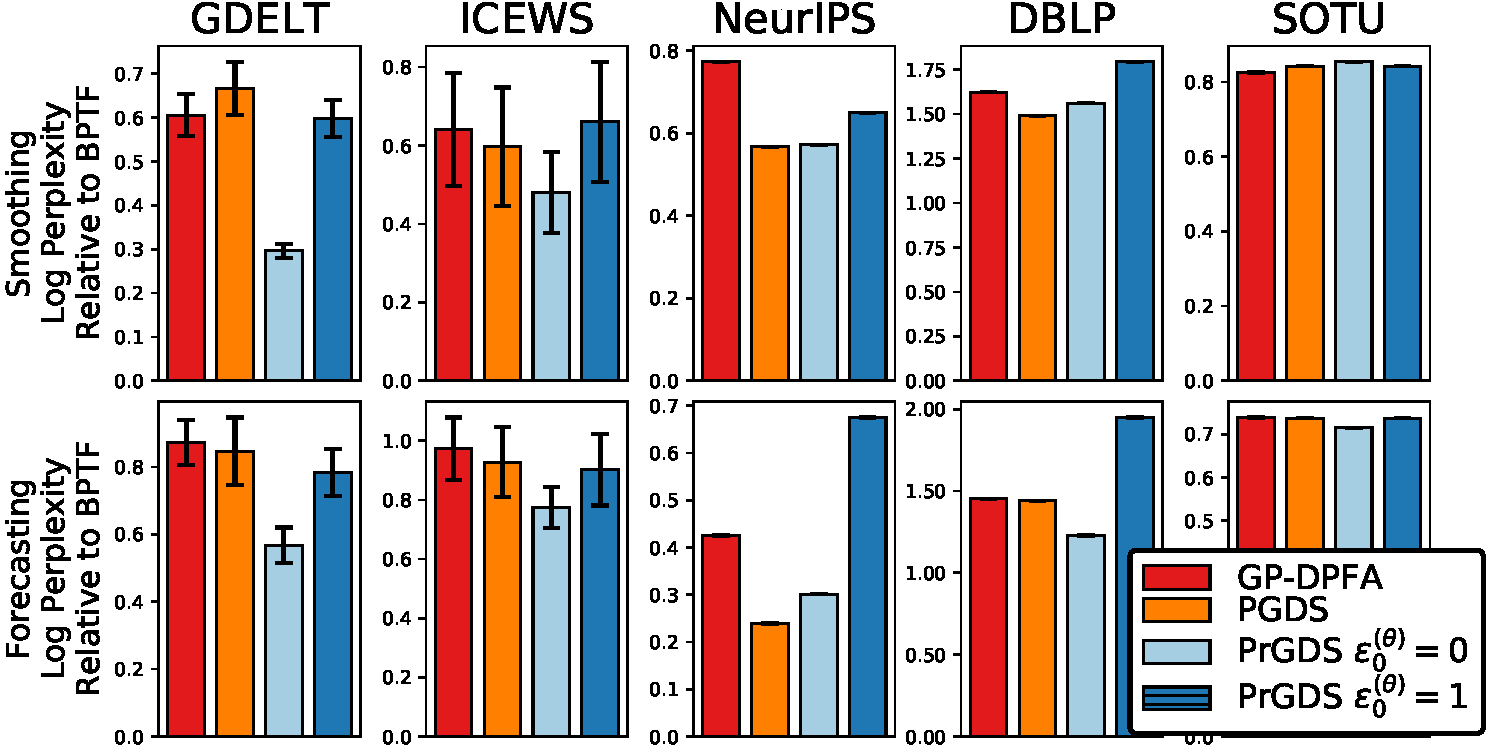
\includegraphics[width=0.669\linewidth]{../../results/matrices/new_matrix_results.pdf}}\hfill
% 
\subfigure[Tensor empirical studies.]
{\label{fig:tensor_results}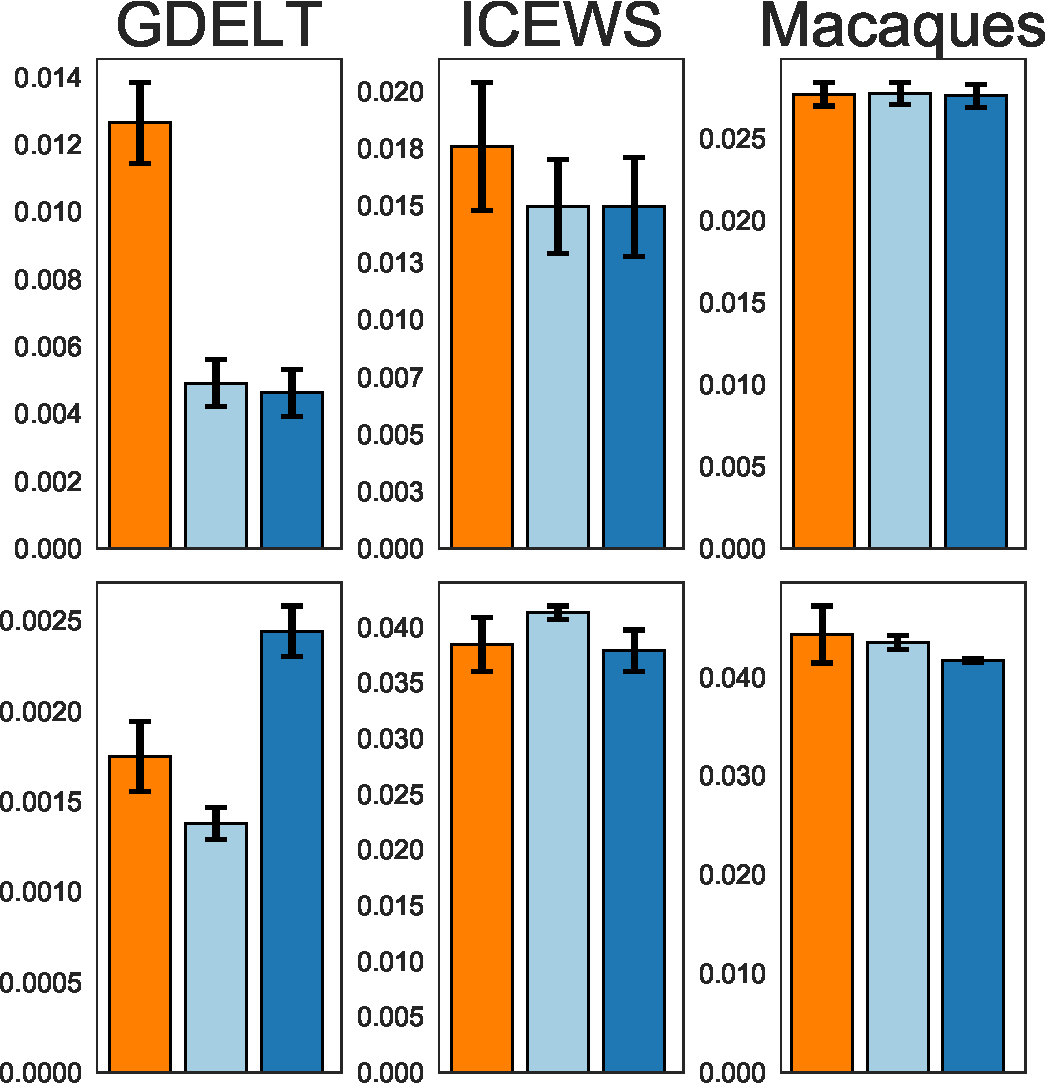
\includegraphics[width=0.32\linewidth]{../../results/tensors/new_tensor_results.pdf}}\vspace{-0.5em}
\caption{\label{fig:empirical}\footnotesize The smoothing (top row) and forecasting (bottom row) performance of each model is measured by log-perplexity---where \emph{lower is better}---divided by the log-perplexity of a non-dynamic baseline, BPTF \cite{schein2015bayesian}.~\looseness=-1}\vspace{-2em}
\end{figure*}

We've seen how the Poisson--gamma--Poisson motif of the PrGDS (see \cref{sec:recursion}) yields a more tractable (see \cref{fig:comparison}) and more flexible (see \cref{sec:bg}) model family than previous work. This motif also encodes a unique inductive bias that we empirically test by comparing the PrGDS to the Poisson--gamma dynamical system (PGDS) \cite{schein2016poisson}. The PGDS is the pure gamma analog to the PrGDS, as we see by comparing \cref{eq:rg1,eq:pgds}---comparing these models thus isolates the impact of the Poisson--gamma--Poisson motif. The PGDS was only previously introduced to model a $T \ttimes V$  \emph{matrix} $Y$ of sequentially observed $V$-dimensional vectors $\boldsymbol{y}^{\mathsmaller{(1)}},\dots, \boldsymbol{y}^{\mathsmaller{(T)}}$. To compare to it, we generalize the PGDS to $M$-mode tensors. We have provided our Cython implementation of the generalized PGDS (in addition to the PrGDS) and derive its complete conditionals in the Appendix. We also compare the PrGDS variant with $\epstheta \teq 1$ to the one with $\epstheta \teq 0$, which permits \emph{sparse activations} $\thetakt \teq 0$.~\looseness=-1

\textbf{Setup.} All empirical studies have the following setup: for some data set $\Yten^{\mathsmaller{(1)}},\dots,\Yten^{\mathsmaller{(T)}}$, all of the counts $\Yten^{\mathsmaller{(t)}}$ at randomly selected time steps $t$ are masked. The last two time steps are also always masked. Each model is fit to the masked data using independent chains of MCMC that impute the missing data each at iteration and ultimately return $S$ posterior samples of the latent variables and parameters. The samples are then used to compute the expectations $\mudt$ (as defined in \cref{eq:tensor_likelihood}) of the heldout counts. We distinguish the task of predicting counts in the final time steps when subsequent observed data is unavailable (\emph{forecasting}) from the task of predicting intermediate time steps (\emph{smoothing}). To assess predictive performance we compute log-perplexity as defined---$\log \textrm{Perp}(\Delta) = -\frac{1}{|\Delta|}\sum_{(t,\osubs) \in \Delta} \log \Big[\frac{1}{S}\sum_{s=1}^S \textrm{Pois}\big(\ydt; \musdt \big) \Big]$---where $\Delta$ is the set of multi-indices of the heldout counts and $\musdt$ is the expectation of the heldout count computed from the $s^{\textrm{th}}$ sample. In all studies, we fit a simple non-dynamic baseline---i.e., Bayesian Poisson tensor factorization (BPTF) \cite{schein2015bayesian}---that assumes the data at different time slices are i.i.d.~$y_{\osubs}^{\mathsmaller{(t)}} \tsim \Pois{\mud}$. This model thus fits $\mud$ from training data and predicts it for all heldout time slices. For the dynamic models, we then report their improvement over non-dynamic BPTF by dividing their log-perplexity by BTPF's.~\looseness=-1 

\textbf{Matrices.} We first replicated the empirical studies on $T\ttimes V$ dynamic \emph{matrices} (i.e., 2-mode tensors) reported by Schein et al.~(2016) \cite{schein2016poisson}. These studies followed the setup described above and compared the PGDS to GP-DPFA \cite{acharya2015nonparametric}, a simple dynamic baseline that we describe in \cref{sec:bg}. The matrices in these studies are based on three text corpora---NeurIPS papers~\cite{neuripscorpus}, DBLP abstracts~\cite{dblp}, and State of the Union (SOTU) speeches~\cite{sotu}---where $\yvt$ is the number of times word $v$ occurs in time step $t$, and two international events data sets---GDELT \cite{leetaru2013gdelt} and ICEWS \cite{boscheeicews}---where $\yvt$ is the number of times sender--receiver pair $v$ interacted during time step $t$. We obtained the matrices and random masks along with the original results for both PGDS and GP-DPFA from the authors and ran the PrGDS with the same MCMC settings they describe (see their paper for details \cite{schein2016poisson}) and BTPF (which uses variational inference) on all matrices and masks. We display the results in \cref{fig:matrix_results}.~\looseness=-1

\textbf{Tensors.} We obtained tensor data from two international events data sets---GDELT and ICEWS---wherein a count $y_{\mathsmaller{i \xrightarrow{a}j}}^{\mathsmaller{(t)}}$ is the number of times country $i$ took action $a$ towards country $j$ during time step $t$. These counts form a sequence of 3-mode tensors of size $V \ttimes V \ttimes A$ for $V \teq 249$ countries and $A \teq 20$ actions. For both data sets, we treat months as time steps, where for GDELT we consider the date range 2003--2008 (thus, $T \teq 72$) and for ICEWS we consider 1995--2013 ($T \teq 228$). 

We also obtained neuroscience data of multielectrode recordings of macaque monkey motor cortices from Williams et al.~(2018)~\cite{williams2018unsupervised}. In this data, a count $y^{\mathsmaller{(t)}}_{ij}$ is the number of times neuron $i$ fired in trial $j$ during time step $t$. These counts form a sequence of matrices each of size $N \ttimes S$ where $N \teq 100$ is the number of neurons and $S \teq 1,716$ is the number of trials. We consider each time step to be a 20 millisecond interval which yields $T \teq 162$. 

For each of the three tensors, we randomly generated two masks that each hold out six time steps in the range $t \in [2, T\tm 2]$ as well as the last two time steps. For each dynamic model, mask, and tensor, we ran two independent chains of $4,000$ MCMC iterations, saving every $100^{\textrm{th}}$ sample after the first 1,000 to compute heldout log-perplexity; we then also fit BPTF and report the relative improvement over it by the dynamic models in \cref{fig:tensor_results}. Following Schein et al.~(2016), we set $K \teq 100$ for all models.~\looseness=-1

\begin{figure*}[t]
\centering
% 
\subfigure[\footnotesize Latent activation structure inferred from neural spike counts in macaque cortex data by the PrGDS. \emph{Right:} Comparison of the $K \ttimes T$ state matrix $\Theta$ inferred by the sparse vs. non-sparse PrGDS. The rows $k$ are sorted by which time step $t$ had the largest $\thetakt$---the banded structure shows that components activate within short durations. White cells correspond to $\thetakt\teq 0$, which only the sparse PrGDS represent. \emph{Left:} Alternative visualization of the rows of~$\Theta$. The sparsity of each vector is provided in the legend. This visualization shows that latent factors are bursty and temporally localized, suggesting that neurons may be tuned to specific periods of the trial.~\looseness=-1]  
{
\label{fig:macaque}
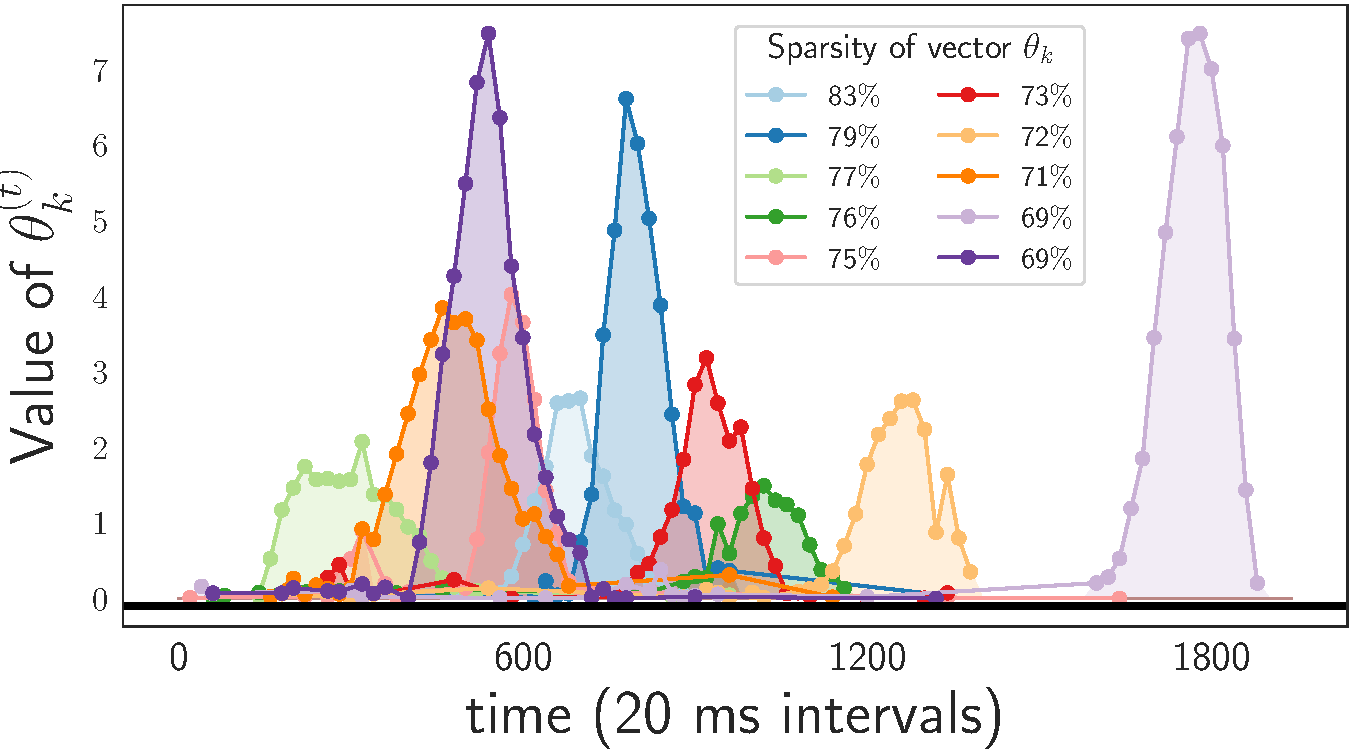
\includegraphics[width=0.49\linewidth]{../../results/tensors/monkeybrains/macaque_components_eps0.pdf}
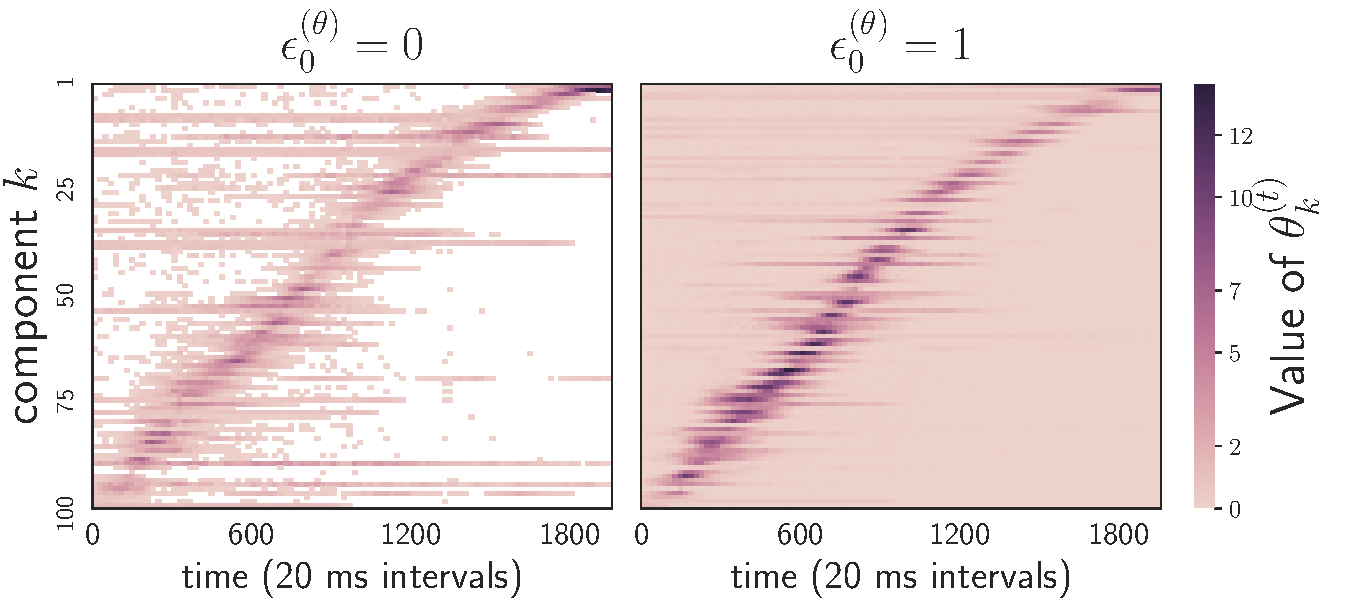
\includegraphics[width=0.49\linewidth]{../../results/tensors/monkeybrains/macaque_heat.pdf}
}\hfill
% 
% 
\subfigure[\footnotesize Two components inferred by the sparse PrGDS from ICEWS data---the blue component was found by other models, the red component was not. The red component is specific to South Sudan, as can be seen by visualizing the largest values of the factor vectors $\boldsymbol{\phi}_k^{\mathsmaller{(m)}}$ for the sender $m \teq 1$ and receiver $m\teq 2$ modes (\emph{bottom row, red}). South Sudan was not a country until July 2011. The activation vector (\emph{top}) is thus sparse---$\thetakt \teq 0$ at 94\% of time steps (months) prior to July 2011 (and 83\% overall). By contrast, the blue component represents Southeast Asian relations, which are persistently active. The sparse PrGDS can infer both temporally-persistent latent structure that other models infer (blue), as well as temporally-localized or bursty structure that other models do not (red).~\looseness=-1]
{
\label{fig:sudan}
% 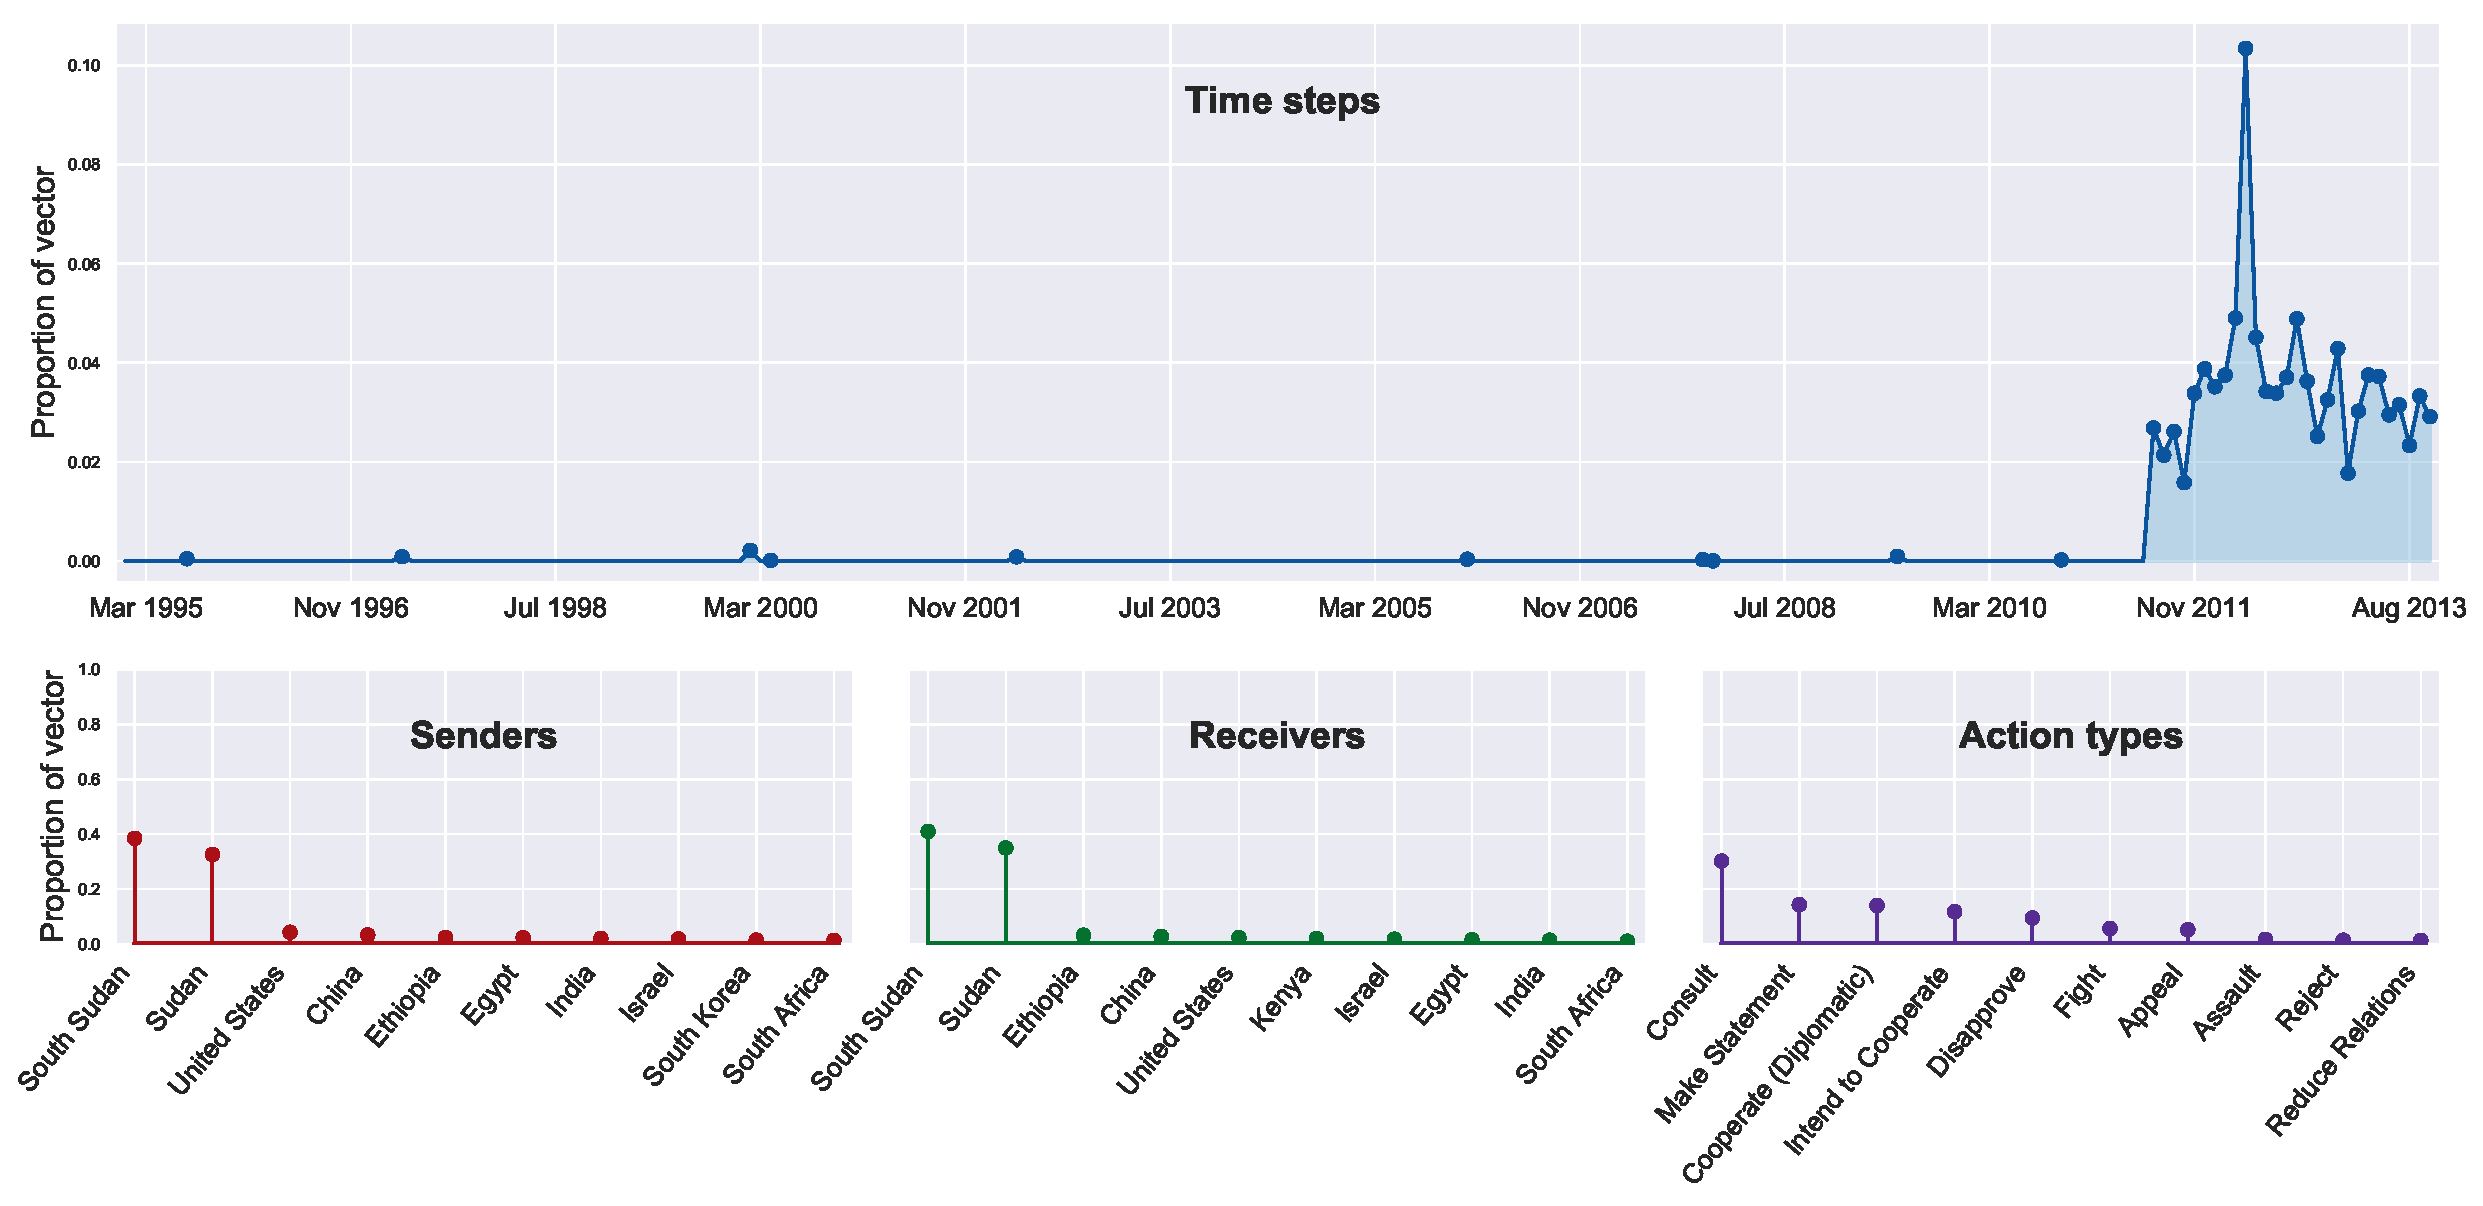
\includegraphics[width=\linewidth]{../../fig/components/icews/zero-ordering/new_plots/eps0-component-0.pdf}
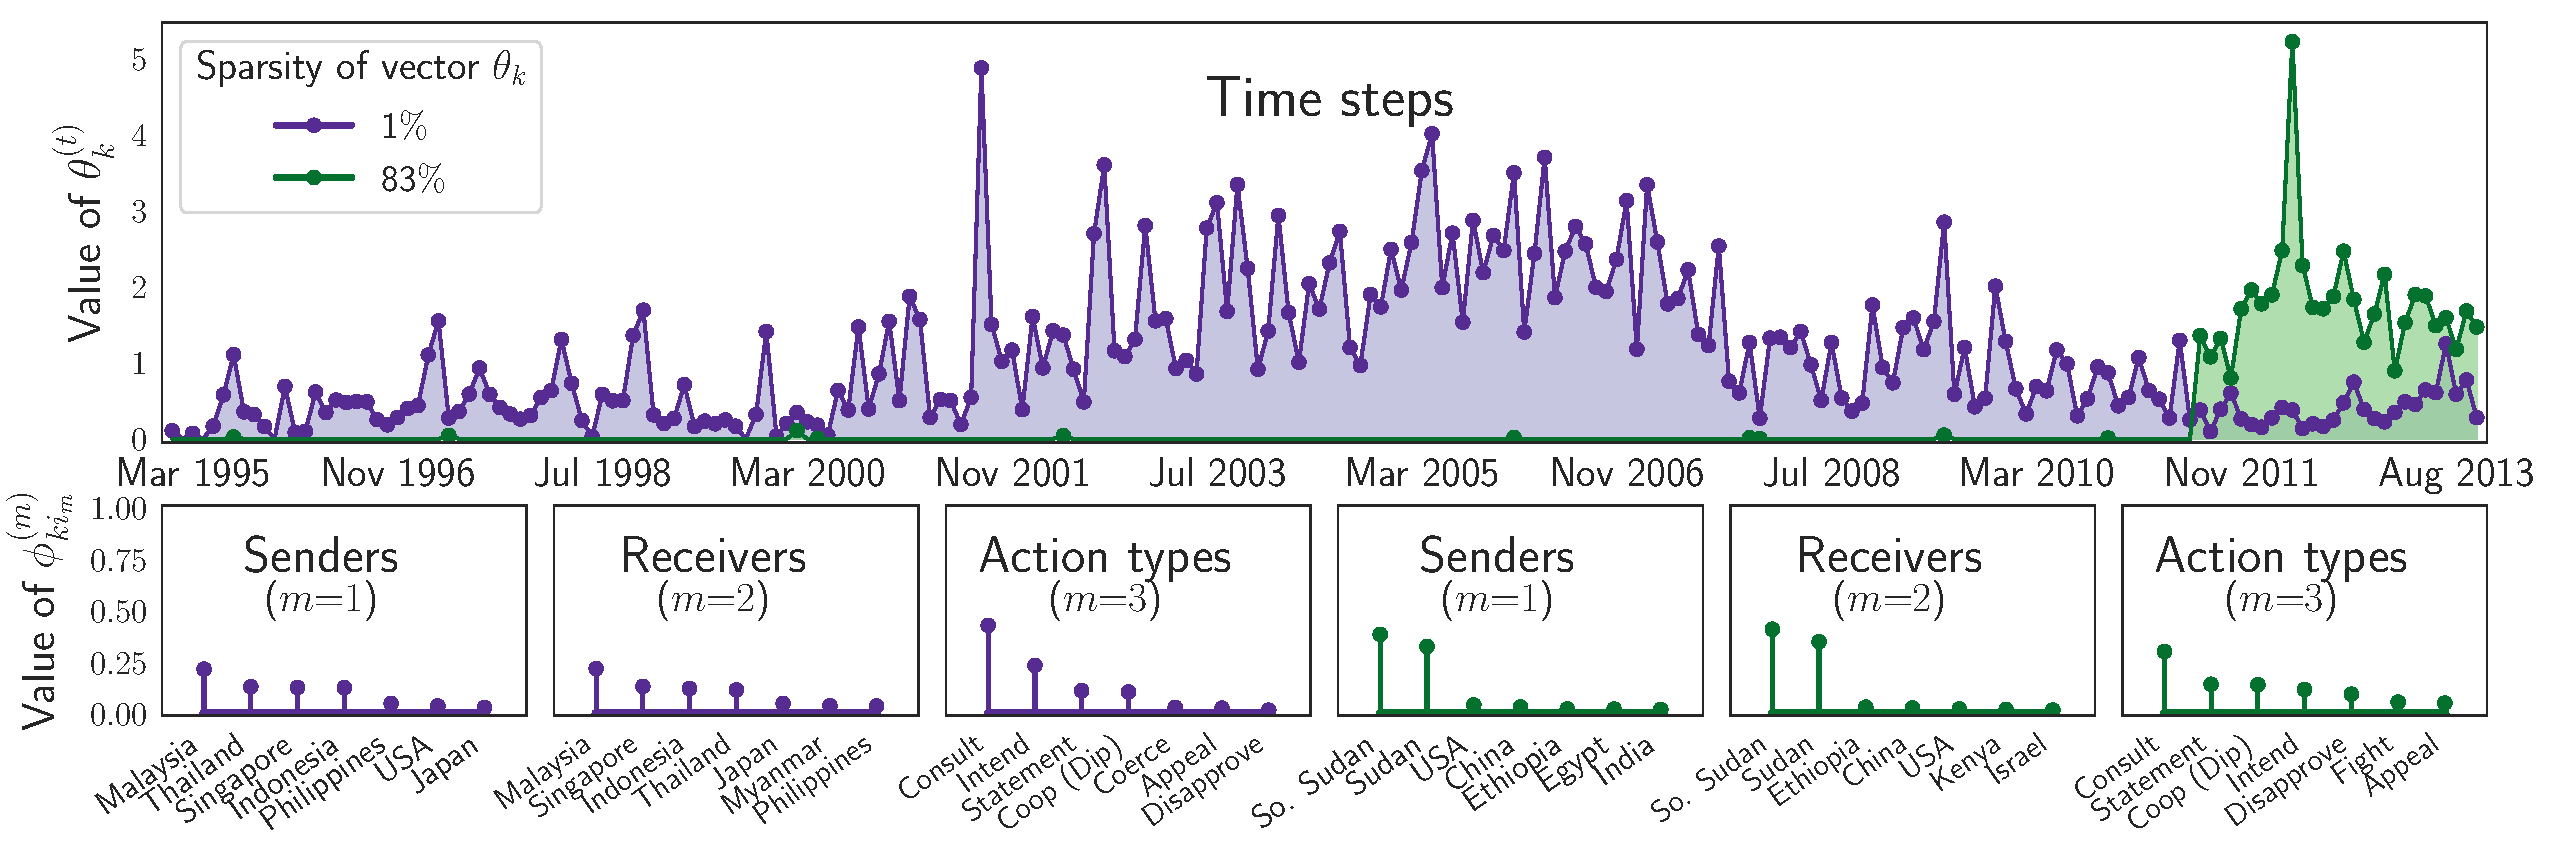
\includegraphics[width=\linewidth]{../../fig/components/icews/zero-ordering/double_plots/eps0-components72-0.pdf}
}
% 
\caption{\label{fig:exploratory} Sparse representations of macaque cortex activity (\cref{fig:macaque}) and ICEWS events (\cref{fig:sudan}).}\vspace{-1em}
\end{figure*}

\textbf{Discussion.} A PrGDS variant obtained the lowest perplexity of all models in ten of the 16 studies (i.e., subplots in \cref{fig:empirical}). The sparse PrGDS obtained lower perplexity than the non-sparse PrGDS in nine studies, sometimes dramatically lower. We conjecture that the better performance of the sparse PrGDS can be explained by the expectation of future states $\boldsymbol{\theta}^{\mathsmaller{(t)}}$ given in \cref{eq:expectation}---when $\epstheta \!>\! 0$ this expectation includes an additive bias term which grows as we forecast further time steps. When $\epstheta \teq 0$ the bias term vanishes and the expectation matches the analogous one for the PGDS, given in \cref{eq:pgds}.~\looseness=-1 

We also performed a qualitative comparison of the different models and found that the sparse PrGDS infers sparse bursty latent structure that the other models do not. We provide a qualitative comparison of the structure inferred by both PrGDS variants from macaque cortex data in \cref{fig:macaque}. In \cref{fig:sudan} we visualize two components---a temporally-persistent one (blue) and a bursty one (red)---that the sparse PrGDS inferred from international events data. While both the non-sparse PrGDS and PGDS found a version of the blue component, neither found the red one. We describe in the Appendix how we align the inferred components across models and provide examples of well-aligned components. We found several instances of bursty components inferred by the sparse PrGDS that could not be meaningfully aligned to any component inferred by the other models.~\looseness=-1


\vspace{-0.25em}\section{Conclusion}\vspace{-0.5em} A novel modeling motif---Poisson--gamma--Poisson recursions---allows us to construct the Poisson-randomized gamma dynamical system, a tractable and expressive model for sequentially observed count tensors. A variant of the PrGDS permits a truly sparse latent representation that is both qualitatively appealing and provides a natural inductive bias for sparse and bursty count time series.

% \begin{figure*}[t]
% \centering
% % 
% \subfigure[\footnotesize Activation vectors $\boldsymbol{\theta}_k$ inferred by the sparse PrGDS.~\looseness=-1]  
% {\label{fig:components}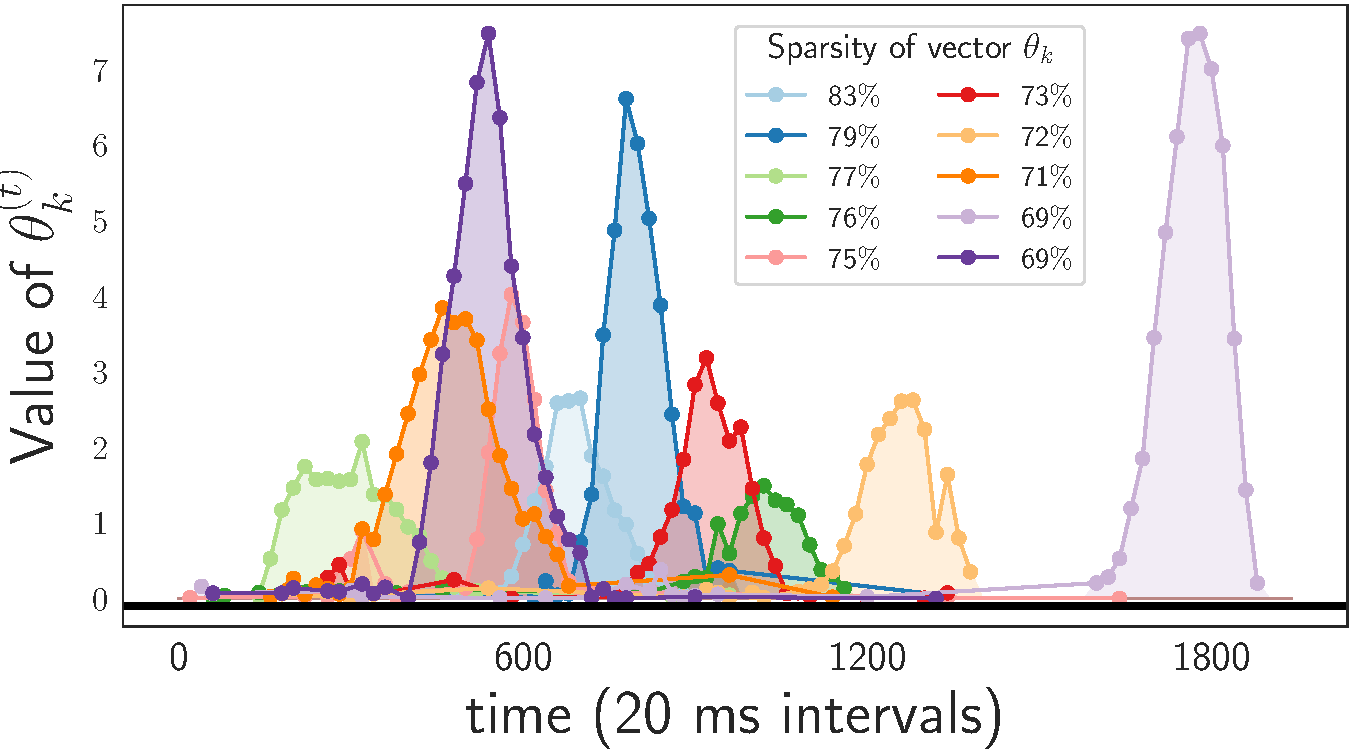
\includegraphics[width=0.49\linewidth]{../../results/tensors/monkeybrains/macaque_components_eps0.pdf}}\hfill
% % 
% \subfigure[\footnotesize The full matrix $\Theta$ inferred by both PrGDS variants.~\looseness=-1]
% {\label{fig:heat}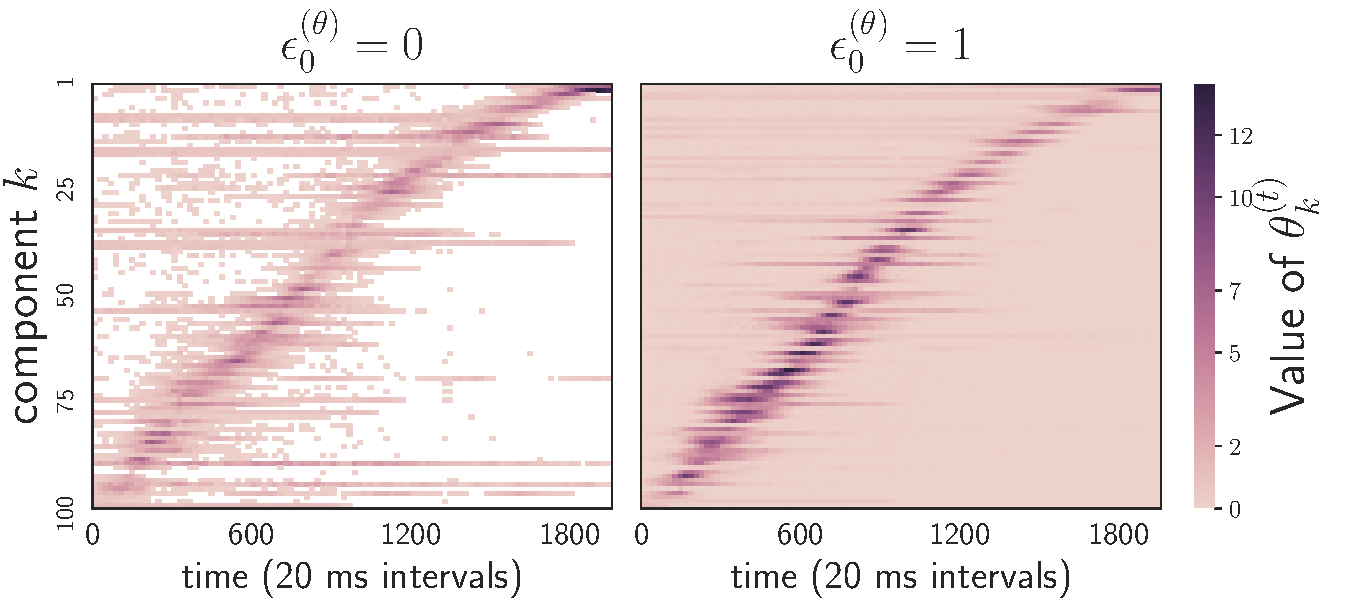
\includegraphics[width=0.49\linewidth]{../../results/tensors/monkeybrains/macaque_heat.pdf}} \vspace{-0.5em}
% % 
% \caption{\label{fig:macaque} \footnotesize Two views of $\Theta$ inferred on Macaque tensor data. \cref{fig:heat} compares the $K \ttimes T$ state matrix inferred by the two PrGDS variants: $\epstheta \teq 0$ (sparse) vs. $\epstheta \teq 1$. The components $k$ are sorted according to which time step $t$ had the largest $\thetakt$---the visible banded structure suggests they both infer components that activate within specific short durations. White cells correspond to exact zeros $\thetakt\teq 0$---the PrGDS can represent truly sparse activation structure when $\epstheta \teq 0$. The $k^{\textrm{th}}$ row $\boldsymbol{\theta}_k$ is the $T$-length activation vector for component $k$---\cref{fig:components} provides an alternative visualization for ten of the sparssest activation vectors inferred by the sparse PrGDS. They collectively depict temporally localized and bursty neuronal spiking dynamics in accordance with neuroscientific accounts.~\looseness=-1}
% \end{figure*}


% \begin{figure*}[b]
% \centering
% 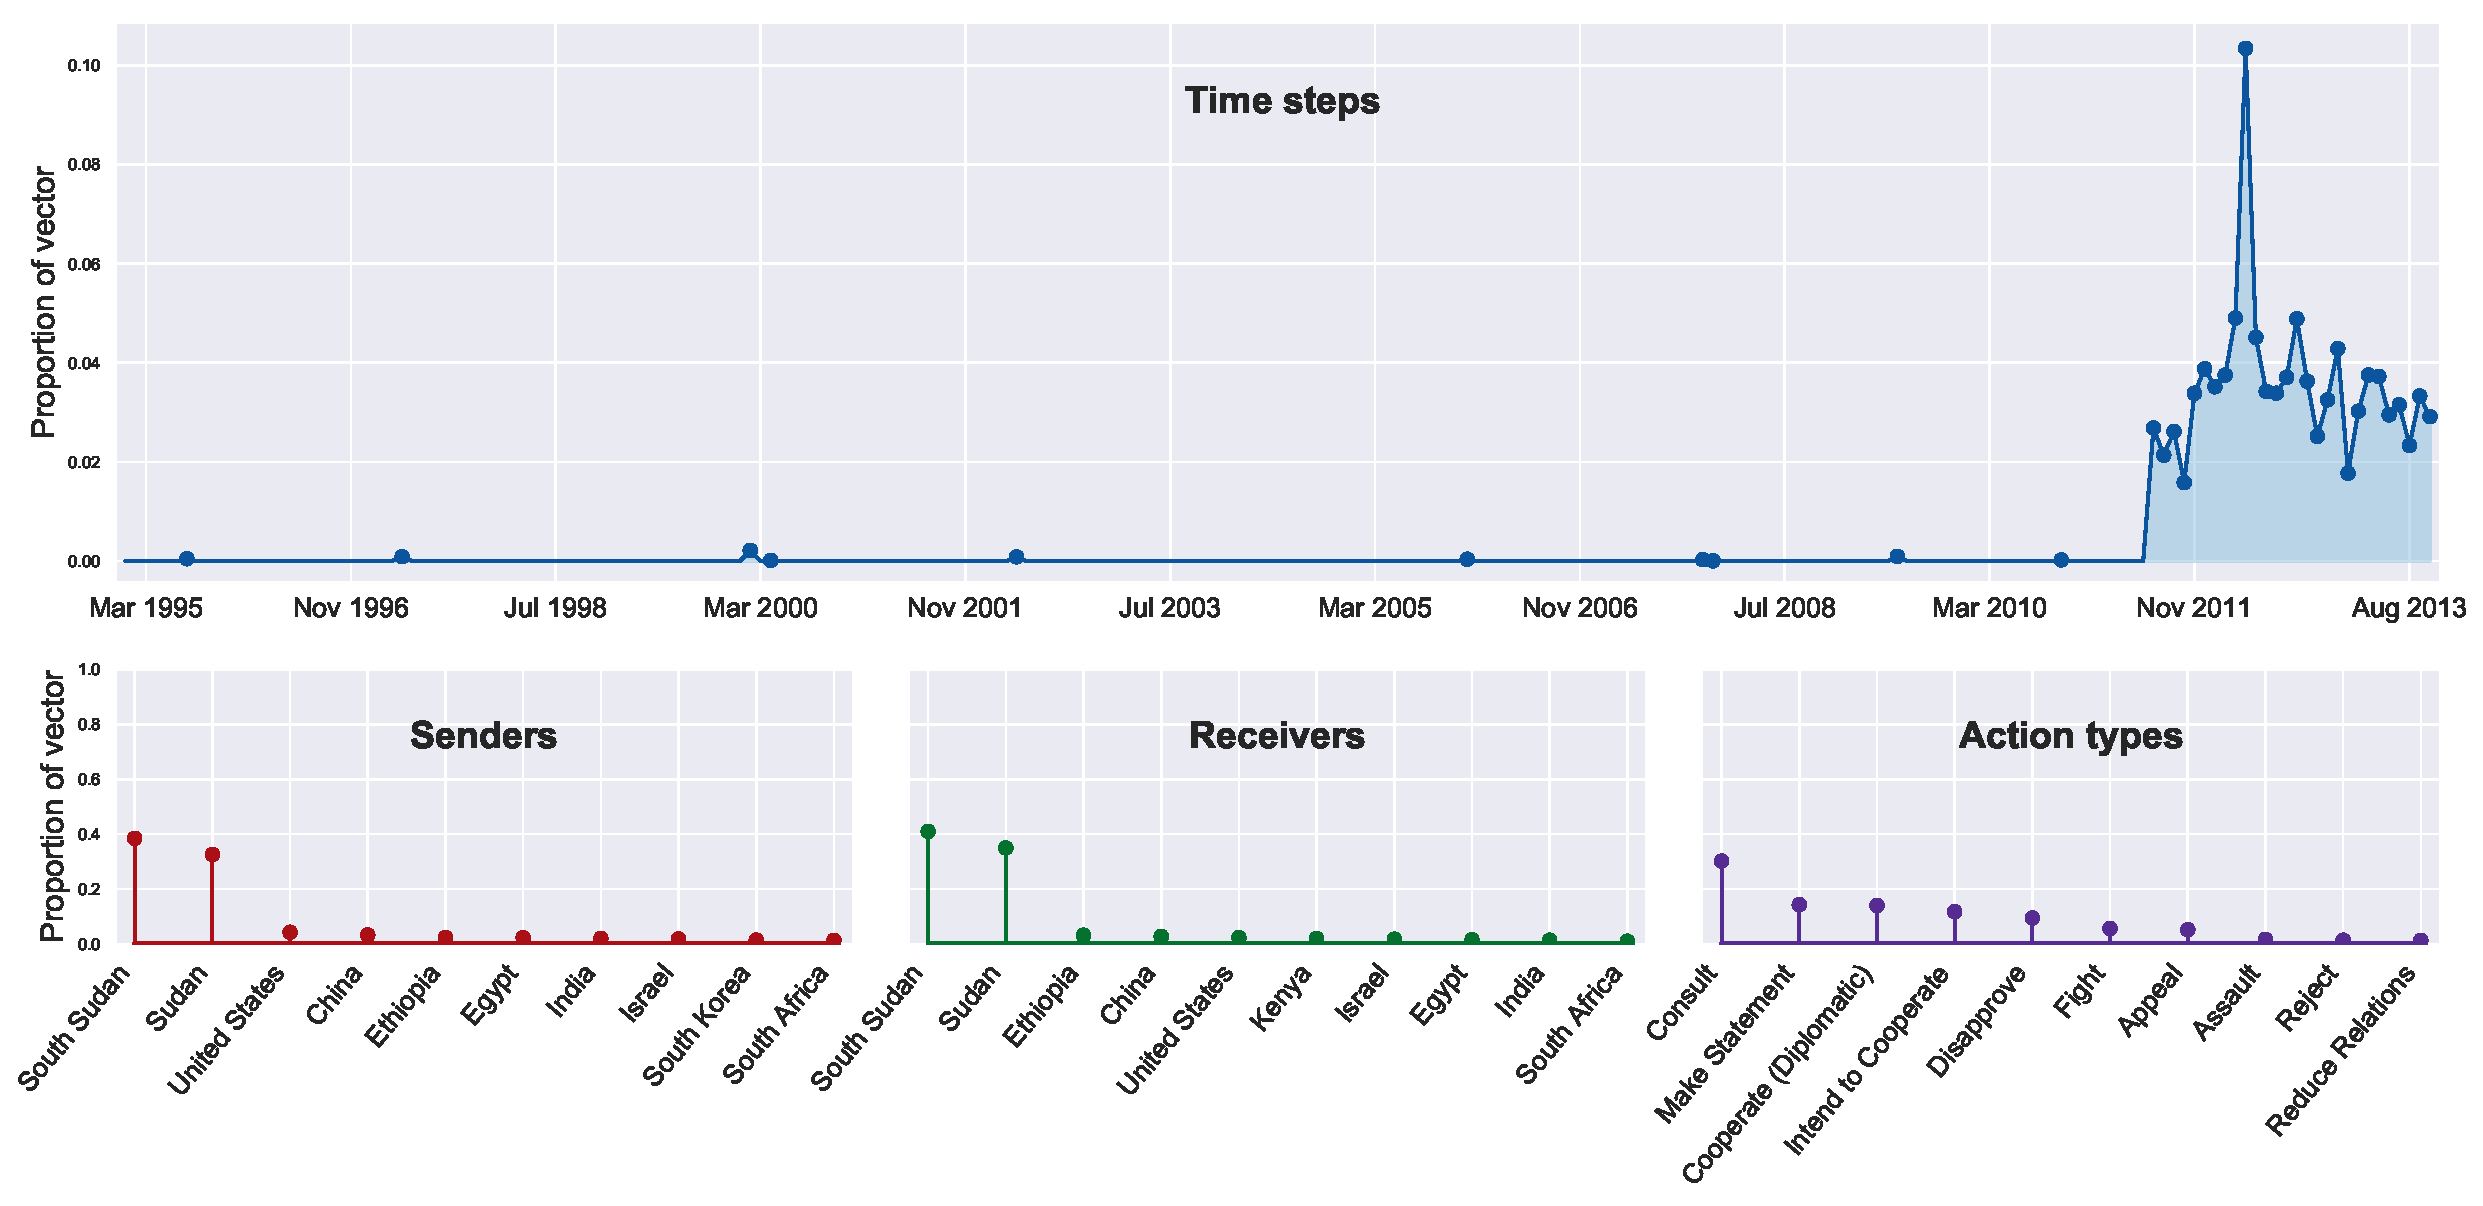
\includegraphics[width=\linewidth]{../../fig/components/icews/zero-ordering/new_plots/eps0-component-0.pdf}
% \caption{\footnotesize \label{fig:sudan} A variant of the PrGDS is capable of inferring true sparsity in its continuous latent states. When fit to dynamic tensor data of country--country interactions, this variant inferred the following component. \emph{Top row:} 94\% of the time steps (months) prior to July 2011 exhibit an inferred latent state value of exactly zero $\thetakt \teq 0$. \emph{Bottom left and middle:} This component mainly summarizes events involving South Sudan, a country that did not exist until July 2011. No other variant of the PrGDS found a component dedicated to South Sudan; we speculate that the sparse variant's unique inductive bias allows it surface patterns in the data that are highly localized in time.~\looseness=-1}
% \end{figure*}




% \section{Discussion}
% \begin{itemize}
% \item $\epstheta = 0$ is better as suggested by \cref{eq:expectation}. 
% \item 
% \end{itemize}
% \label{sec:conc}
\pagebreak
\bibliographystyle{unsrt}
\bibliography{references}

\end{document}